\documentclass[journal]{IEEEtran}
\usepackage[brazil]{babel}
\usepackage[utf8]{inputenc}
\usepackage{bm, amsmath, amssymb, graphics, setspace}
\usepackage{tikz}
\usetikzlibrary{scopes}
\usetikzlibrary{calc,patterns,angles,quotes}
\usepackage{amssymb}
\usepackage{float}
\usepackage{graphicx}
\usepackage{hyperref}
\usepackage{siunitx}
\usepackage{subfig}
\usepackage{tabularx}
\usepackage{multicol}
\usepackage[export]{adjustbox}
\usepackage{enumerate}
\usepackage{euscript}

\newcommand\scalemath[2]{\scalebox{#1}{\mbox{\ensuremath{\displaystyle #2}}}}

\begin{document}
       
\title{\huge Laboratório de Controle e Automação I
	   \huge \\ Projeto Desafio: Rotor Duplo}

\author{Emerson Alves \\ Victor Moraes}

\maketitle

\begin{abstract}
	Este relatório descreve a prática de controle da planta de um rotor duplo. O sistema é composto por duas hélices, semelhante a um helicóptero, sendo uma no sentido horizontal e outra no vertical. O intuito do presente trabalho foi realizar o controle de ambos graus de liberdade da planta: ângulos de arfagem e de guinada. Para tal, realizou-se identificação do sistema para cada entrada e para cada saída. Assim foram obtidas quatro funções de transferência que aproxima o sistema real. Tal modelo foi validado por meio de simulações na planta. Foi realizado o projeto de um desacoplador e controladores PID foram projetados para controle de arfagem e guinada. Esses controladores foram simulados nos modelos e posteriormente testado na planta.
\end{abstract}

\IEEEpeerreviewmaketitle

\section{Introdução}
	Uma das aplicações de controle na aeronáutica mais importantes é o controle da orientação espacial de uma aeronave, a fim de alterar a trajetória do veículo em voo. Os ângulos controlados são: em relação ao eixo horizontal, ângulo de arfagem; em relação ao eixo vertical: ângulo de guinada; e em relação ao sentido longitudinal da aeronave, o ângulo de rolagem. 
Em helicópteros comerciais tais controles são realizados atuando na velocidade dos rotores e ângulos das pás, controlando empuxo, arfagem e guinada.

O dispositivo didático utilizada nesta prática é o sistema rotor duplo de múltiplas entradas e múltiplas saídas (MIMO), que é uma simplificação de um helicóptero e produzida pela \textit{Feedback}. O controle de tal planta deve possuir dois controladores, sendo cada um dependente de ambas entradas. Contudo, é possível desacoplar as entradas e eliminar o efeito cruzado, isto é, o efeito em que uma entrada, afeta a saída oposta, permitindo o controle de um sistema MIMO.

\begin{figure}[H]
    \centering
    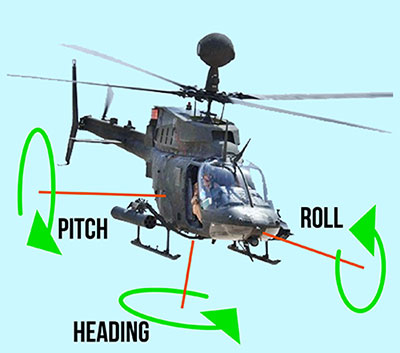
\includegraphics[width=0.30\textwidth]{figures/pitch-roll-heading.jpg}
    \caption{Orientação espacial de uma aeronave: arfagem (\textit{pitch}), rolagem (\textit{roll}) e guinada (\textit{heading}).}
    \label{fig:helicoptero}
\end{figure}


\section{Descrição da Planta}\label{Sec:DescricaoPlanta}
	O sistema é composto por dois rotores de velocidade variáveis, sendo uma hélice horizontal e outra vertical, acoplado em uma haste com dois graus de liberdade que por sua vez está conectada a uma outra haste com contra-peso.
A planta possui duas variáveis de entrada, que são as tensões de alimentação de cada rotor, fornecidas pela unidade eletrônica, que recebe uma referência de $-2.5$ a $\SI{2.5}{\volt}$ do controlador. Também possui duas variáveis a serem controladas, correspondente aos dois graus de liberdade: ângulo de arfagem e angulo de guinada, sendo sensoreadas, cada uma, por \textit{encoders} incrementais, lidos pela unidade de aquisição de dados e enviados ao controlador \cite{ManualRotor}.

\begin{figure}[H]
    \centering
    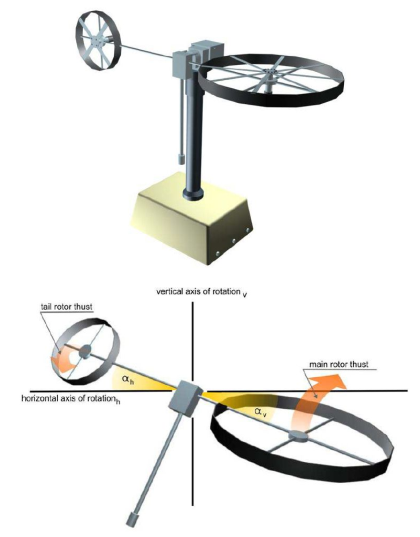
\includegraphics[width=0.30\textwidth]{figures/twin_rotor.PNG}
    \caption{Dispositivo \textit{Twin rotor MIMO System}.}
    \label{fig:TwinRotor}
\end{figure}

No sistema físico está presente a perturbação de fluxos de ar externos e turbulências. Como não-linearidades, tem-se o atraso da aceleração do rotor e de seu empuxo. O torque de arfagem depende de forma não-linear da orientação espacial.

Tem-se como variável controlada o ângulo de arfagem (\textit{pitch angle}), responsável pelo movimento vertical do rotor dianteiro. A tensão aplicada ao rotor é a variável manipulada. O \textit{set-point} ou referência é o ângulo de arfagem desejado, que nessa prática foi expresso em sinais do tipo degrau, senoide e rampa. A variável medida foi o ângulo de arfagem real do rotor (resposta do sistema).

% Para realizar o controlador, optou-se por operar em uma faixa próxima da posição horizontal, a fim de aproximar a planta para um sistema linear.


\section{Especificação do Desempenho Desejado}\label{Sec:EspecifDesemp}
	Os requisitos de desempenho no domínio do tempo adotados para o controle de pitch foram:

\begin{enumerate}
    \item \textit{Overshoot} máximo percentual: $M_{p} \leq 30\%$;
    \item Tempo de acomodação: $t_{2\%} \leq \SI{20}{\s}$; e
    \item Erro nulo em estado estacionário para entradas do tipo degrau.
\end{enumerate}

Os requisitos de desempenho no domínio do tempo adotados para o controle de yaw foram:

\begin{enumerate}
    \item \textit{Overshoot} máximo percentual: $M_{p} \leq 20\%$;
    \item Tempo de acomodação: $t_{2\%} \leq \SI{10}{\s}$; e
    \item Erro nulo em estado estacionário para entradas do tipo degrau.
\end{enumerate}


Tais requisitos introduziram restrições que delimitaram uma região de suposto desempenho satisfatório no plano complexo $s$, e foram consideradas no projeto dos controladores.


\section{Modelagem Matemática da Planta}\label{Sec:ModelagemPlanta}
	
Os modelos matemáticos que descrevem o comportamento do ângulo de arfagem (\textit{pitch}), ângulo de guinada (\textit{yaw}), \textit{cross-pitch} e \textit{cross-yaw}, foram obtidos pelo método de identificação em malha aberta. Que consiste na aplicação de um sinal de excitação na planta e coleta e análise de sua resposta a essa entrada. O modelo matemático é então obtido relacionando-se o sinal de saída com o sinal de entrada por meio de um sistema padrão de 2ª ordem ou modificações dele.

Como se trata de um sistema MIMO, foi necessário identificar quatro FTs, a saber: a do ângulo de arfagem $G_{\Phi}$ (\textit{pitch}), a do ângulo de guinada $G_{\Psi}$ (\textit{yaw}), a do \textit{cross-pitch} $G_{cp}$ e a do \textit{cross-yaw} $G_{cy}$. A representação do sistema em diagrama de blocos é mostrada na Figura \ref{fig:IdentificaMIMOSystem}.

\begin{figure}[H]
    \centering
    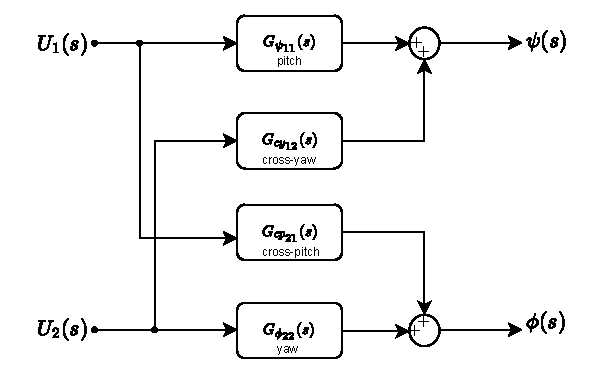
\includegraphics[width=0.48\textwidth]{figures/Identificacao/Identificacao_MIMO.pdf}
    \caption{Diagrama de blocos do sistema MIMO.}
    \label{fig:IdentificaMIMOSystem}
\end{figure}

\noindent onde $U_{1}(s)$ e $U_{2}(s)$ representam as tensões aplicadas nos motores que controlam os rotores do \textit{pitch} e do \textit{yaw}, e $\Phi(s)$ e $\Psi(s)$ os ângulos de arfagem e de guinada, respectivamente.

%%%%%%%%%%%%%%%%%%%%%%%%%%%%%%%%%%%%%%%%%%%%%%%%%%%%%%%%%%%%%
\subsection{\textbf{Modelagem do ângulo de arfagem (\textit{pitch})}}

Para identificar o modelo do ângulo de arfagem, foram aplicados dois degraus, um de amplitude $\SI{1.36}{\volt}$ e outro de amplitude $\SI{0.34}{\volt}$. A soma dessas amplitudes corresponde à tensão que deixa o rotor paralelo ao chão. A resposta do ângulo do rotor a essa entrada é mostrada na Figura \ref{fig:IdentificacaoPitchAngle}.

\begin{figure}[H]
    \centering
    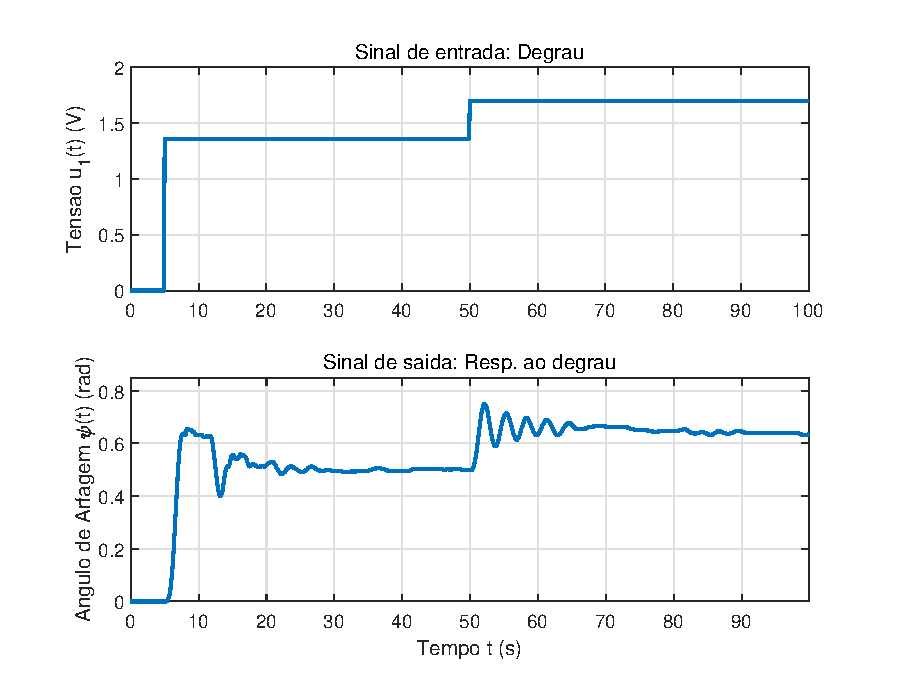
\includegraphics[width=0.48\textwidth]{figures/Identificacao/IdentificaPitchInicial.eps}
    \caption{Identificação do modelo do ângulo de arfagem (\textit{pitch}).}
    \label{fig:IdentificacaoPitchAngle}
\end{figure}

Para a identificação do modelo, apenas a resposta ao segundo degrau foi considerada. Pois, para variações de baixa amplitude, o sistema não sai do entorno de seu ponto de operação e responde, portanto, de forma linear. 

A resposta obtida é típica de um sistema padrão de segunda ordem subamortecido $( 0 < \zeta \leq 1)$. Considerando a existência de tempo-morto, a função de transferência de interesse é da forma
\begin{equation}\label{eq:FTPitch}
    G_{\psi}(s) = \frac{\Psi(s)}{U_{1}(s)} = \frac{k w_{n}^2 e^{-\tau_d s}}{s^2 + 2 \zeta w_{n} s + w_{n}^2}
\end{equation}
\noindent onde $k$ é o ganho estático, $w_n$ a frequência natural de oscilação (em $\si{\radian/\s}$), $\zeta$ é o coeficiente de amortecimento e $\tau_d$ o tempo-morto em $\si{s}$.

Com $t_{i}$ e $t_{i+1}$ os instantes de tempo em que ocorrem dois picos consecutivos na resposta, a frequência amortecida pode ser aproximada por
$$ w_d = \frac{2 \pi}{T} \approx \frac{2 \pi}{t_{i+1} - t_i} = \frac{2 \pi}{30.2 - 27.1} = \SI{2.0268}{\radian/\s} $$
\noindent já um valor inicial para $\zeta$, de acordo com \cite{aguirre2004}, pode ser obtido contando-se o número $N$ de picos visíveis na resposta
$$ \zeta \approx \frac{0.6}{N} = \frac{0.6}{5} = 0.12 $$
\noindent e o ganho estático
$$ k = \frac{\Delta \psi}{\Delta u_{1}} = \frac{0.7486 - 0.7148}{0.34} = 0.0994 $$
Após sobrepor as respostas da planta e do modelo, removendo a condição inicial (deslocado para a origem), tal como mostrado na Figura \ref{fig:IdentificacaoPitchAngleDesloc}, os valores do coeficiente de amortecimento e do ganho foram ajustados para
$$ \zeta = 0.06 \quad\text{e}\quad k = 0.462 $$
e para esse novo valor de $\zeta$, obteve-se
$$ w_{n} = \frac{w_{d}}{\sqrt{1 - \zeta^2}} = \SI{2.03049}{\radian/\s} $$
O valor do atraso foi obtido por inspeção: $\tau_{d} \approx \SI{0.5}{\s}$.

\begin{figure}[H]
    \centering
    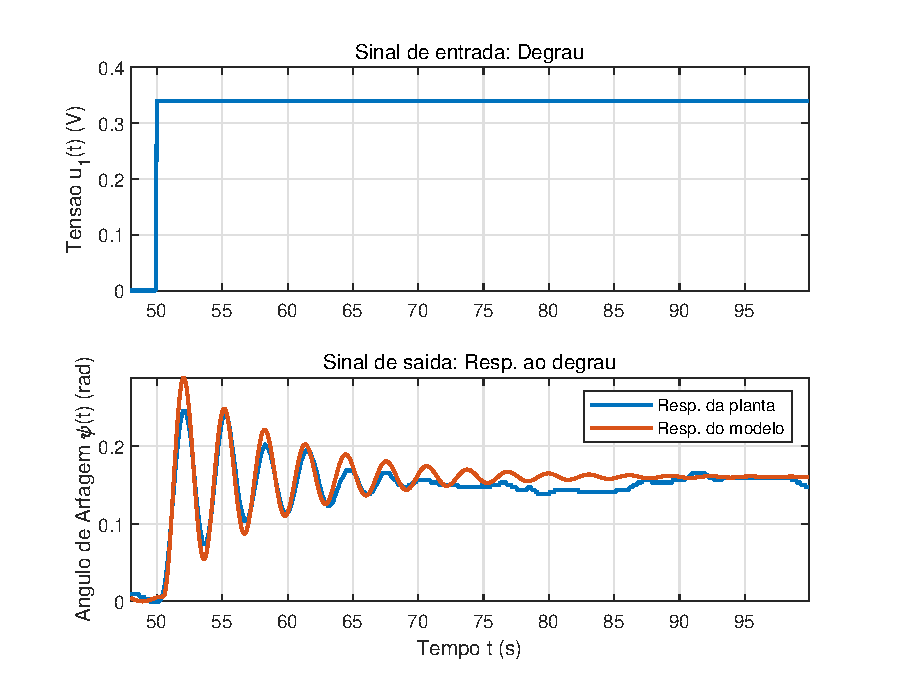
\includegraphics[width=0.48\textwidth]{figures/Identificacao/IdentificaPitchFinal.eps}
    \caption{Sinal original e modelo identificado para o ângulo de arfagem (\textit{pitch}).}
    \label{fig:IdentificacaoPitchAngleDesloc}
\end{figure}

Assim, o modelo matemático que descreve o comportamento do ângulo de arfagem é dado por
\begin{equation}\label{eq:FTModeloIDPitch}
    G_{\psi}(s) = \frac{\Psi(s)}{U_{1}(s)} = \frac{1.905 e^{-0.5 s}}{s^2 + 0.2437 s + 4.123}
\end{equation}

%%%%%%%%%%%%%%%%%%%%%%%%%%%%%%%%%%%%%%%%%%%%%%%%%%%%%%%%%%%%%%%%%%%%%%%%%%%%%%%%%%%
%%%%%%%%%%%%%%%%%%%%%%%%%%%%%%%%%%%%%%%%%%%%%%%%%%%%%%%%%%%%%%%%%%%%%%%%%%%%%%%%%%%
%%%%%%%%%%%%%%%%%%%%%%%%%%%%%%%%%%%%%%%%%%%%%%%%%%%%%%%%%%%%%%%%%%%%%%%%%%%%%%%%%%%
\subsection{\textbf{Modelagem do ângulo de guinada (\textit{yaw})}}

Para identificar o modelo do ângulo de guinada, foi aplicado um degrau de amplitude $\SI{0.6}{\volt}$. Um valor baixo de tensão foi necessário devido a excursão limitada da rotação do eixo do rotor da cauda, impedindo que se chegasse ao fim de curso e prejudicasse a qualidade do sinal medido do ângulo. A resposta do ângulo do rotor da cauda a essa entrada é mostrada na Figura \ref{fig:IdentificacaoYawAngleInicial}.

\begin{figure}[H]
    \centering
    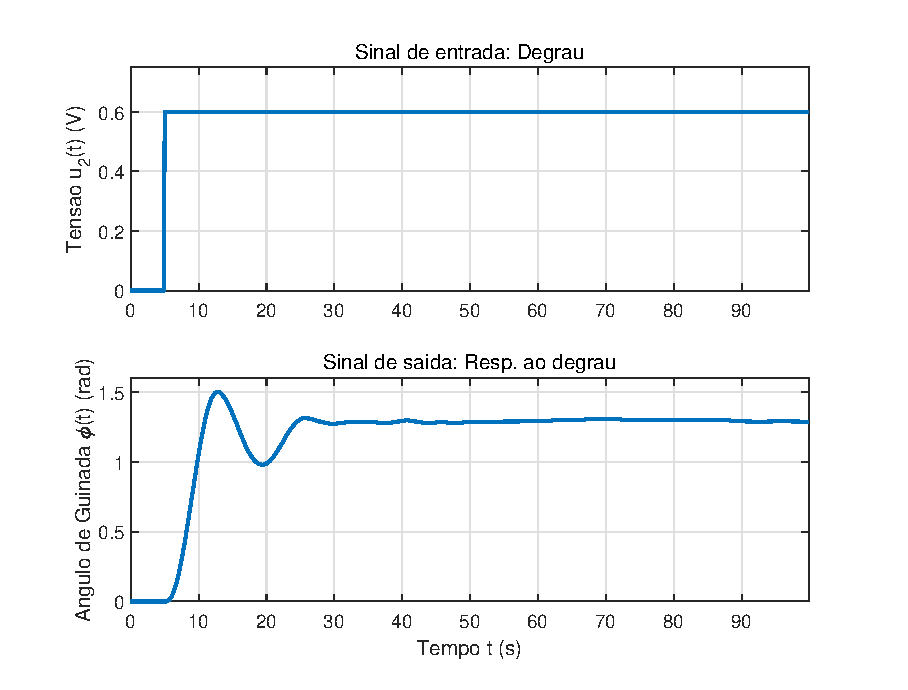
\includegraphics[width=0.48\textwidth]{figures/Identificacao/IdentificaYawInicial.eps}
    \caption{Identificação do modelo do ângulo de guinada (\textit{yaw}).}
    \label{fig:IdentificacaoYawAngleInicial}
\end{figure}

A resposta obtida é, novamente, típica de um sistema padrão de segunda ordem subamortecido $( 0 < \zeta \leq 1)$. Considerando a existência de tempo-morto, a função de transferência de interesse é da forma
\begin{equation}\label{eq:FTYaw}
    G_{\phi}(s) = \frac{\Phi(s)}{U_{2}(s)} = \frac{k w_{n}^2 e^{-\tau_d s}}{s^2 + 2 \zeta w_{n} s + w_{n}^2}
\end{equation}
\noindent onde $k$ é o ganho estático, $w_n$ a frequência natural de oscilação (em $\si{\radian/\s}$), $\zeta$ é o coeficiente de amortecimento e $\tau_d$ o tempo-morto em $\si{s}$.

Com $t_{i}$ e $t_{i+1}$ os instantes de tempo em que ocorrem dois picos consecutivos no ângulo de guinada, a frequência amortecida foi aproximada por
$$ w_d = \frac{2 \pi}{T} \approx \frac{2 \pi}{t_{i+1} - t_i} = \frac{2 \pi}{25.5-12.8} = \SI{0.5026}{\radian/\s} $$
\noindent o valor inicial para $\zeta$, \cite{aguirre2004}, foi obtido a partir do número $N$ de picos visíveis no sinal de saída
$$ \zeta \approx \frac{0.6}{N} = \frac{0.6}{2} = 0.3 $$
\noindent já o ganho estático
$$ k = \frac{\Delta \phi}{\Delta u_{2}} = \frac{1.5 - 1.285}{0.6} = 0.3583 $$
Esses parâmetros foram então ajustados por meio da sobreposição das respostas da planta e do modelo, a fim de se obter um melhor ajuste. Os valores finais para $\zeta$, $w_{n}$, $k$ foram
$$ \zeta = 0.42 \quad\text{e}\quad k = 1.65 \quad\text{e}\quad w_{n} = \SI{0.47}{\radian/\s} $$
O valor do atraso, obtido por inspeção, foi $\tau_{d} \approx \SI{0.5}{\s}$.

Assim, o modelo matemático que descreve o comportamento do ângulo de guinada é dado por
\begin{equation}\label{eq:FTModeloIDYaw}
    G_{\phi}(s) = \frac{\Phi(s)}{U_{2}(s)} = \frac{0.3645 e^{-0.5 s}}{s^2 + 0.3948s + 0.2209}
\end{equation}
O resultado da sobreposição do modelo identificado com o sinal original do ângulo de guinada é mostrado na Figura \ref{fig:IdentificacaoYawAngleFinal}.

\begin{figure}[H]
    \centering
    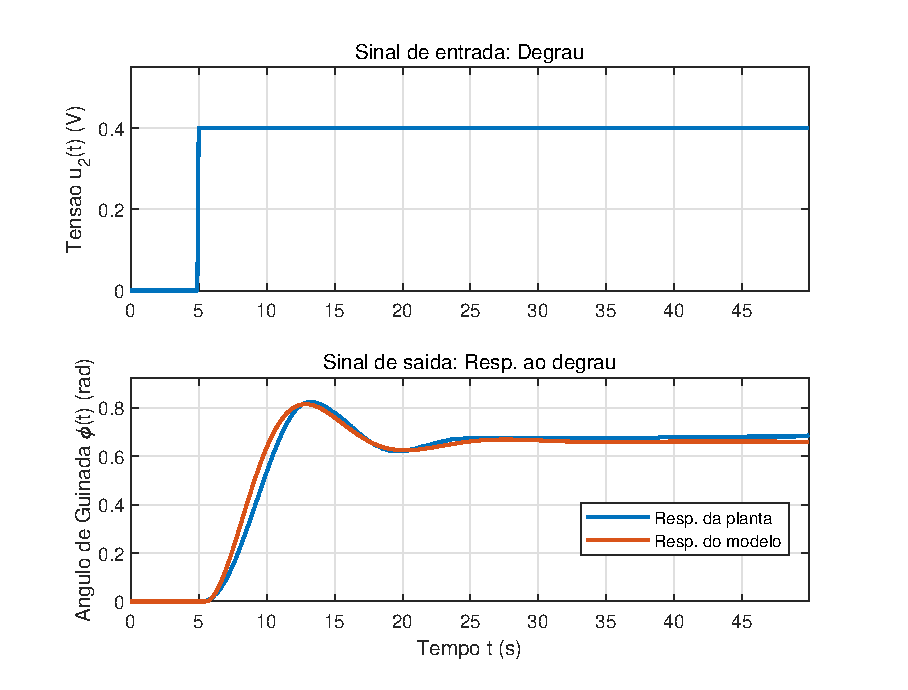
\includegraphics[width=0.48\textwidth]{figures/Identificacao/IdentificaYawFinal.eps}
    \caption{Sinal original e modelo identificado para o ângulo de guinada (\textit{yaw}).}
    \label{fig:IdentificacaoYawAngleFinal}
\end{figure}

%%%%%%%%%%%%%%%%%%%%%%%%%%%%%%%%%%%%%%%%%%%%%%%%%%%%%%%%%%%%%%%%%%%%%%%%%%%%%%%%%%%
%%%%%%%%%%%%%%%%%%%%%%%%%%%%%%%%%%%%%%%%%%%%%%%%%%%%%%%%%%%%%%%%%%%%%%%%%%%%%%%%%%%
%%%%%%%%%%%%%%%%%%%%%%%%%%%%%%%%%%%%%%%%%%%%%%%%%%%%%%%%%%%%%%%%%%%%%%%%%%%%%%%%%%%
\subsection{\textbf{Modelagem do \textit{cross-pitch}}}

Para identificação do modelo do \textit{cross-pitch}, que relaciona a tensão aplicada no rotor dianteiro (principal) com a variação do ângulo de guinada (\textit{yaw}), foi aplicada uma tensão em $u_{1}$ (rotor dianteiro), na forma de um degrau de amplitude $\SI{1}{\volt}$. Esse sinal de entrada e a resposta do ângulo \textit{yaw}, para $u_{2} = 0$, tensão no rotor da cauda nula, são mostradas na Figura \ref{fig:IdentificacaoCrossPitchInicial}.

\begin{figure}[H]
    \centering
    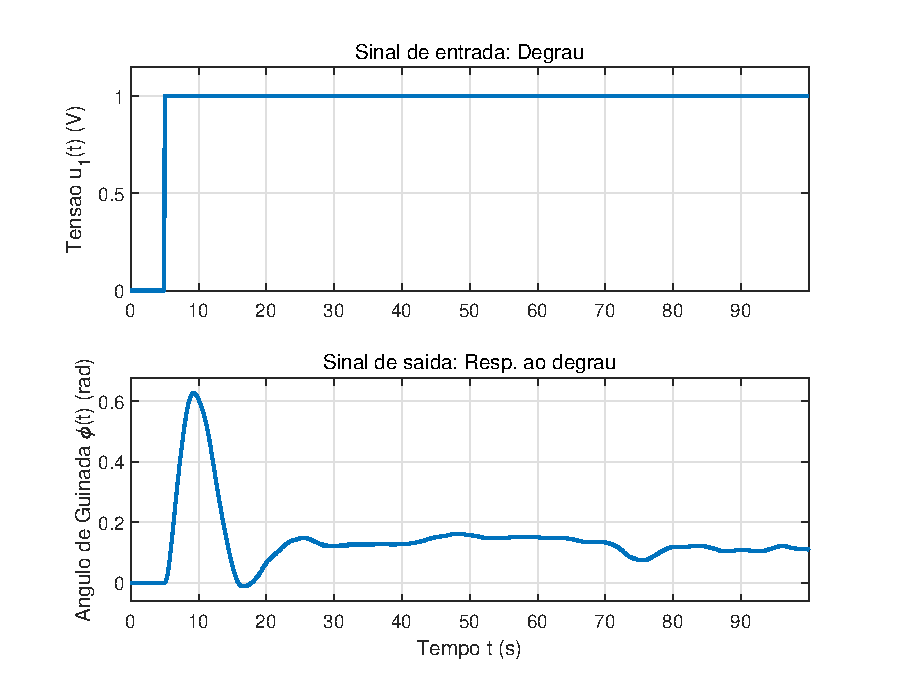
\includegraphics[width=0.48\textwidth]{figures/Identificacao/IdentificaCrossPitchInicial.eps}
    \caption{Identificação do modelo do \textit{cross-pitch}.}
    \label{fig:IdentificacaoCrossPitchInicial}
\end{figure}

Para relacionar esses sinais, buscou-se identificar um modelo da forma
\begin{equation}\label{eq:FTCrossPitch}
    G_{cp}(s) = \frac{\Phi(s)}{U_{1}(s)} = \frac{k w_{n}^2 (a_{1} s + a_{0})e^{-\tau_d s}}{s^2 + 2 \zeta w_{n} s + w_{n}^2}
\end{equation}
\noindent onde $k$ é o ganho estático, $w_n$ a frequência natural de oscilação (em $\si{\radian/\s}$), $\zeta$ é o coeficiente de amortecimento, $\tau_d$ o tempo-morto em $\si{s}$ e $a_{1}$ e $a_{0}$ são os coeficientes do numerador.

Para tanto, foi utilizada a ferramenta de identificação \textit{Ident} do \textit{Matlab}. A partir dos sinais de entrada e saída fornecidos, obteve-se o seguinte modelo para a FT do \textit{cross-pitch}
\begin{equation}\label{eq:FTModeloIDCrossPitch}
    G_{cp}(s) = \frac{\Phi(s)}{U_{1}(s)} = \frac{0.3025(s+0.06162)e^{-s}}{s^2 + 0.2574 s + 0.1437}
\end{equation}
O resultado da sobreposição do modelo identificado na equação \eqref{eq:FTModeloIDCrossPitch} com o sinal original do \textit{cross-pitch} é mostrado na Figura \ref{fig:IdentificacaoCrossPitchFinal}.

\begin{figure}[H]
    \centering
    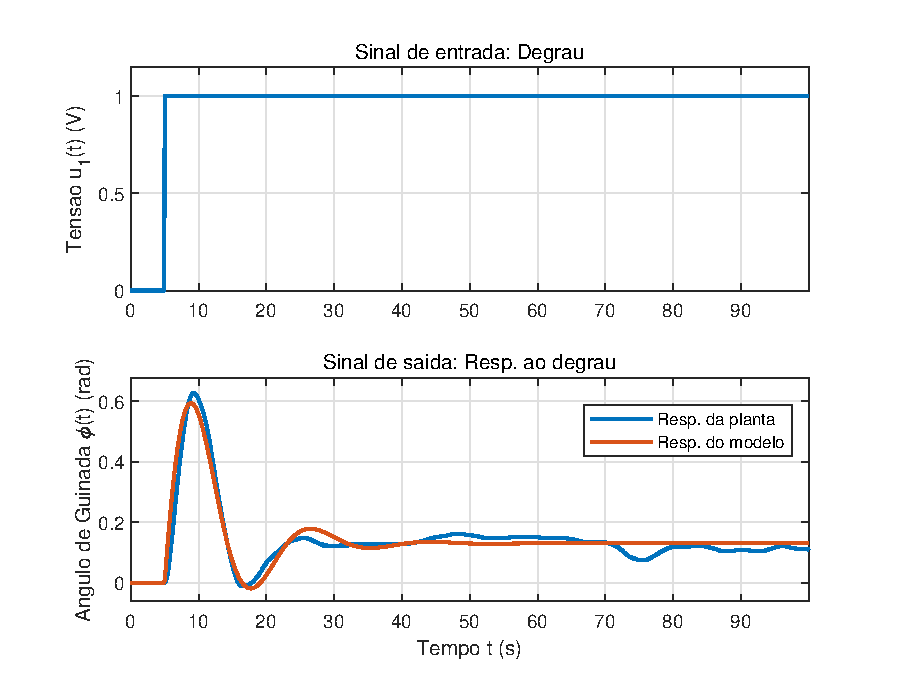
\includegraphics[width=0.48\textwidth]{figures/Identificacao/IdentificaCrossPitchFinal.eps}
    \caption{Sinal original e modelo identificado para o \textit{cross-pitch}.}
    \label{fig:IdentificacaoCrossPitchFinal}
\end{figure}

%%%%%%%%%%%%%%%%%%%%%%%%%%%%%%%%%%%%%%%%%%%%%%%%%%%%%%%%%%%%%%%%%%%%%%%%%%%%%%%%%%%
%%%%%%%%%%%%%%%%%%%%%%%%%%%%%%%%%%%%%%%%%%%%%%%%%%%%%%%%%%%%%%%%%%%%%%%%%%%%%%%%%%%
%%%%%%%%%%%%%%%%%%%%%%%%%%%%%%%%%%%%%%%%%%%%%%%%%%%%%%%%%%%%%%%%%%%%%%%%%%%%%%%%%%%
\subsection{\textbf{Modelagem do \textit{cross-yaw}}}

Já a identificação do modelo do \textit{cross-yaw}, que busca relacionar a tensão aplicada no rotor da cauda com a variação do ângulo de arfagem (\textit{pitch}), se valeu da aplicação de uma tensão em $u_{2}$ (rotor da cauda), na forma de um degrau com amplitude $\SI{0.6}{\volt}$. A Figura \ref{fig:IdentificacaoCrossYawInicial} mostra o sinal de entrada da tensão aplicada e a resposta do ângulo \textit{pitch} para essa entrada, com $u_{1} = 0$, tensão no rotor dianteiro nula.

\begin{figure}[H]
    \centering
    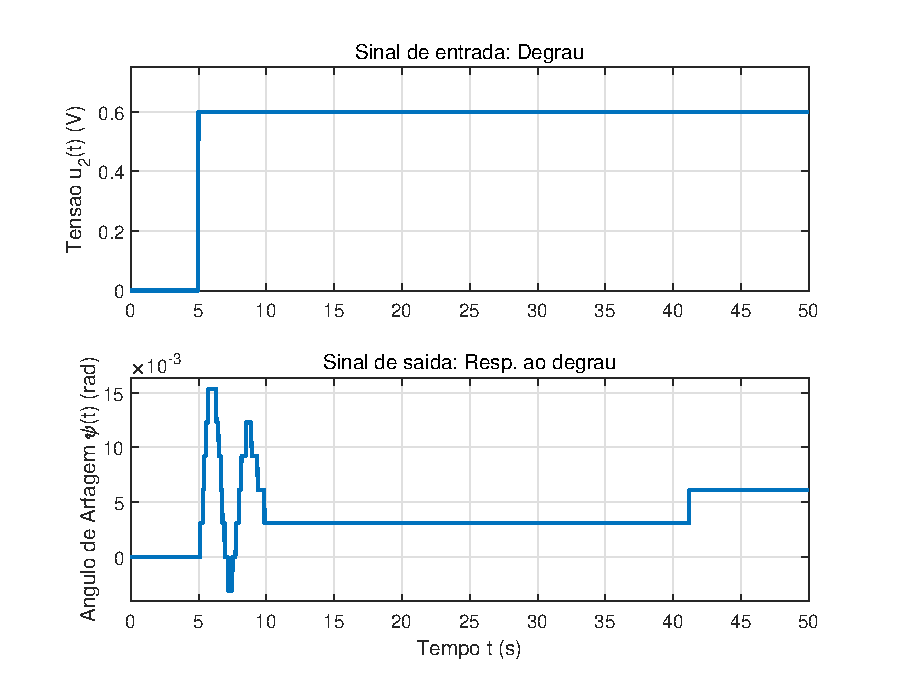
\includegraphics[width=0.48\textwidth]{figures/Identificacao/IdentificaCrossYawInicial.eps}
    \caption{Identificação do modelo do \textit{cross-yaw}.}
    \label{fig:IdentificacaoCrossYawInicial}
\end{figure}

O modelo utilizado para relacionar esses sinais foi da forma
\begin{equation}\label{eq:FTCrossYaw}
    G_{cy}(s) = \frac{\Psi(s)}{U_{2}(s)} = \frac{k w_{n}^2 (a_{1} s + a_{0})e^{-\tau_d s}}{s^2 + 2 \zeta w_{n} s + w_{n}^2}
\end{equation}
\noindent onde $k$ é o ganho estático, $w_n$ a frequência natural de oscilação (em $\si{\radian/\s}$), $\zeta$ é o coeficiente de amortecimento, $\tau_d$ o tempo-morto em $\si{s}$ e $a_{1}$ e $a_{0}$ são os coeficientes do numerador.

Utilizando-se novamente a ferramenta de identificação do \textit{Matlab}, obteve-se o seguinte modelo para a FT do \textit{cross-yaw}, para os sinais de entrada e saída fornecidos
\begin{equation}\label{eq:FTModeloIDCrossYaw}
    G_{cy}(s) = \frac{\Psi(s)}{U_{2}(s)} = \frac{0.0476(s+1.2945)e^{-0.13s}}{s^2 + 0.6339 s + 4.262}
\end{equation}
A Figura \ref{fig:IdentificacaoCrossYawFinal} mostra o resultado da sobreposição do modelo identificado na equação \eqref{eq:FTModeloIDCrossYaw} com o sinal original do \textit{cross-yaw}.

\begin{figure}[H]
    \centering
    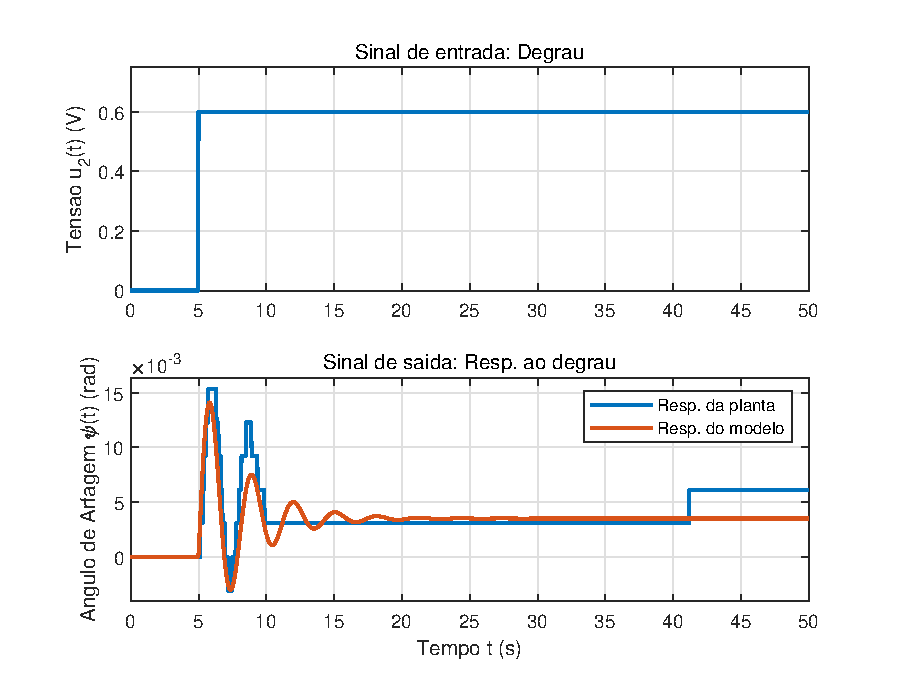
\includegraphics[width=0.48\textwidth]{figures/Identificacao/IdentificaCrossYawFinal.eps}
    \caption{Sinal original e modelo identificado para o \textit{cross-yaw}.}
    \label{fig:IdentificacaoCrossYawFinal}
\end{figure}

%%%%%%%%%%%%%%%%%%%%%%%%%%%%%%%%%%%%%%%%%%%%%%%%%%%%%%%%%%%%%%%%%%%%%%%%%%%%%%%%%%%
%%%%%%%%%%%%%%%%%%%%%%%%%%%%%%%%%%%%%%%%%%%%%%%%%%%%%%%%%%%%%%%%%%%%%%%%%%%%%%%%%%%
%%%%%%%%%%%%%%%%%%%%%%%%%%%%%%%%%%%%%%%%%%%%%%%%%%%%%%%%%%%%%%%%%%%%%%%%%%%%%%%%%%%
\subsection{\textbf{Modelos Identificados}}

Um resumo das FTs identificadas para os ângulos de arfagem, guinada, além do \textit{cross-pitch} e \textit{cross-yaw}, respectivamente, são mostradas nas equações a seguir:

\begin{equation}\tag{\ref{eq:FTModeloIDPitch}}
    G_{\psi}(s) = \frac{\Psi(s)}{U_{1}(s)} = \frac{1.905 e^{-0.5 s}}{s^2 + 0.2437 s + 4.123}
\end{equation}

\begin{equation}\tag{\ref{eq:FTModeloIDYaw}}
    G_{\phi}(s) = \frac{\Phi(s)}{U_{2}(s)} = \frac{0.3645 e^{-0.5 s}}{s^2 + 0.3948s + 0.2209}
\end{equation}

\begin{equation}\tag{\ref{eq:FTModeloIDCrossPitch}}
    G_{{cp}_{21}}(s) = \frac{\Phi(s)}{U_{1}(s)} = \frac{0.3025(s+0.06162)e^{-s}}{s^2 + 0.2574 s + 0.1437}
\end{equation}

\begin{equation}\tag{\ref{eq:FTModeloIDCrossYaw}}
    G_{{cy}_{12}}(s) = \frac{\Psi(s)}{U_{2}(s)} = \frac{0.0476(s+1.2945)e^{-0.13s}}{s^2 + 0.6339 s + 4.262}
\end{equation}

Na próxima seção esses modelos são validados para outros sinais de entrada, ou seja, sinais com características diferentes dos utilizados na fase de identificação.

\section{Validação do Modelo}\label{Sec:ValidacaoModelo}
	
Nesta seção são mostrados os resultados da validação dos modelos obtidos, equações \eqref{eq:FTModeloIDPitch}, \eqref{eq:FTModeloIDYaw}, \eqref{eq:FTModeloIDCrossPitch} e \eqref{eq:FTModeloIDCrossYaw}, para diferentes sinais de entrada.

%%%%%%%%%%%%%%%%%%%%%%%%%%%%%%%%%%%%%%%%%%%%%%%%%%%%%%%%%%%%%%%%%%%
\subsection{\textbf{Validação do Modelo do \textit{pitch}}}

A validação do modelo obtido para o ângulo \textit{pitch}, para sinais de entrada com características diferentes dos utilizados na fase de identificação são mostrados nas Figuras \ref{fig:ValidaPitchDegrau} e \ref{fig:ValidaPitchSenoide}.

A Figura \ref{fig:ValidaPitchDegrau} apresenta a resposta da planta e do modelo a um degrau de amplitude $\SI{0.7}{\volt}$ aplicado no instante $t = \SI{75}{\s}$.

\begin{figure}[H]
    \centering
    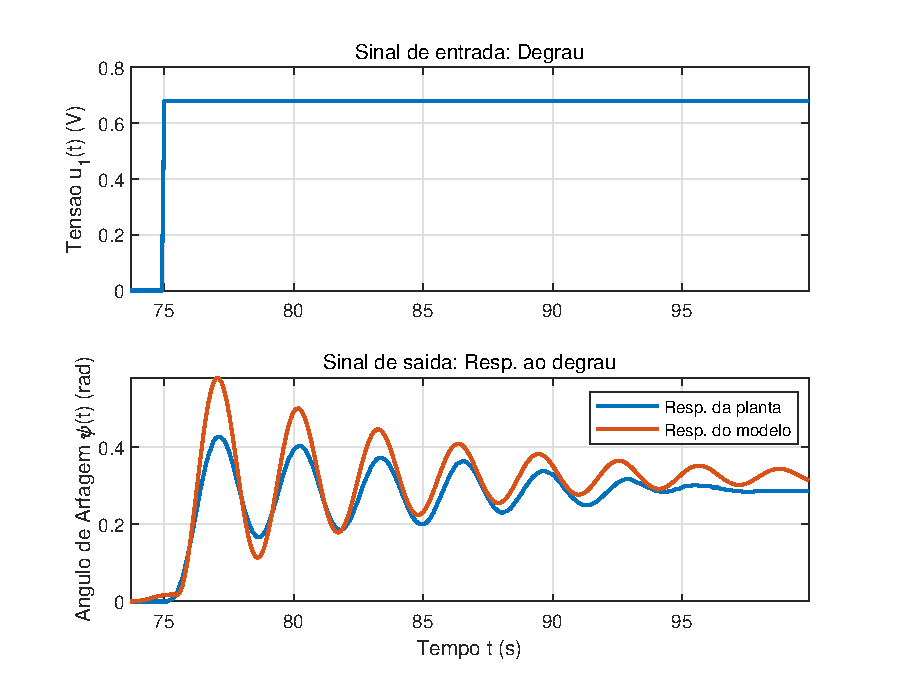
\includegraphics[width=0.45\textwidth]{figures/Validacao/ValidaPitchDegrau.eps}
    \caption{\textit{Pitch}: Sinal de entrada em degrau e resposta da planta e do modelo a essa entrada.}
    \label{fig:ValidaPitchDegrau}
\end{figure}

Já a Figura \ref{fig:ValidaPitchSenoide} mostra a resposta a uma entrada senoidal de amplitude $\SI{0.34}{\volt}$ e frequência $\SI{0.1}{\Hz}$.

\begin{figure}[H]
    \centering
    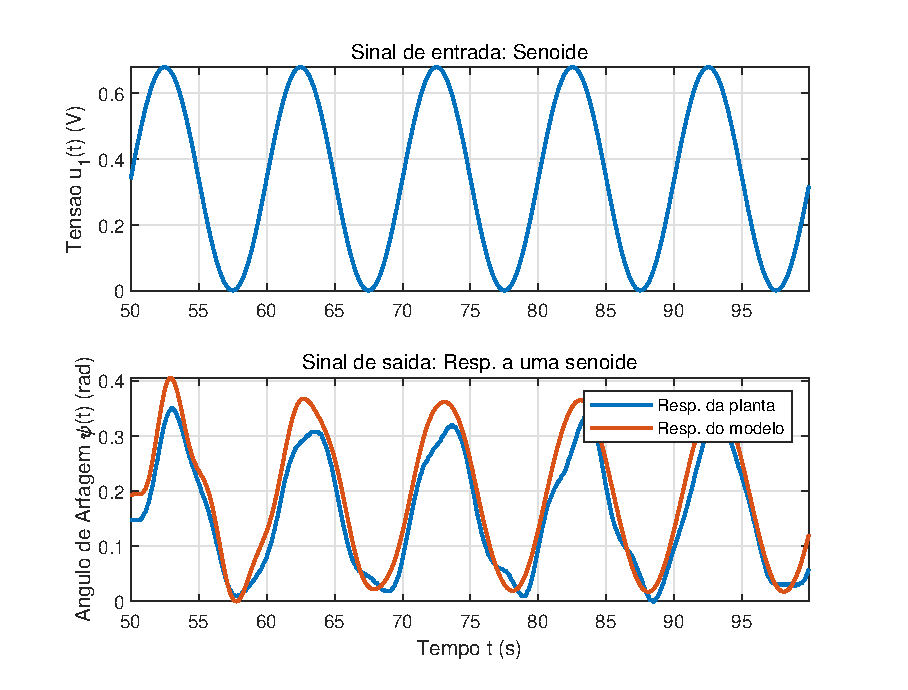
\includegraphics[width=0.45\textwidth]{figures/Validacao/ValidaPitchSenoide.eps}
    \caption{\textit{Pitch}: Sinal de entrada senoidal e resposta da planta e do modelo a essa entrada.}
    \label{fig:ValidaPitchSenoide}
\end{figure}

Pode-se observar pelas respostas obtidas que o modelo se aproxima de forma satisfatória do comportamento da planta, com amplitude, frequência de oscilação e amortecimentos próximos.

%%%%%%%%%%%%%%%%%%%%%%%%%%%%%%%%%%%%%%%%%%%%%%%%%%%%%%%%%%%%%%%%%%%
\subsection{\textbf{Validação do Modelo do \textit{yaw}}}

O modelo obtido para o ângulo \textit{yaw} foi validado também para sinais de entrada do tipo pulso e senoide. Os quais são mostrados nas Figuras \ref{fig:ValidaYawPulso} e \ref{fig:ValidaYawSenoide}.

Na Figura \ref{fig:ValidaYawPulso}, aplicou-se um pulso de amplitude $\SI{0.6}{\volt}$, com período de $T = \SI{50}{\s}$.

\begin{figure}[H]
    \centering
    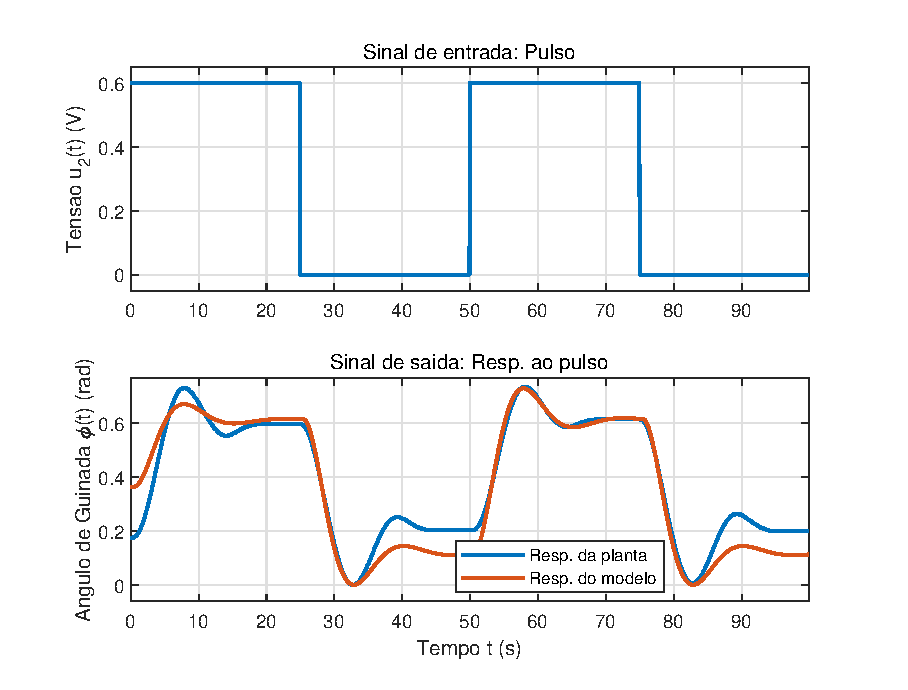
\includegraphics[width=0.48\textwidth]{figures/Validacao/ValidaYawPulso.eps}
    \caption{\textit{Yaw}: Sinal de entrada em pulso e resposta da planta e do modelo a essa entrada.}
    \label{fig:ValidaYawPulso}
\end{figure}

Pode-se observar que o modelo foi capaz de modelar corretamente o comportamento do ângulo de guinada, principalmente em se tratando de degraus positivos, nos quais tanto a amplitude quanto o amortecimento e a frequência ficaram bem ajustados.

Na Figura \ref{fig:ValidaYawSenoide}, o modelo para o \textit{yaw} é validado para uma entrada senoidal de amplitude $\pm \SI{0.3}{\volt}$, com período de $T = \SI{20}{\s}$.

\begin{figure}[H]
    \centering
    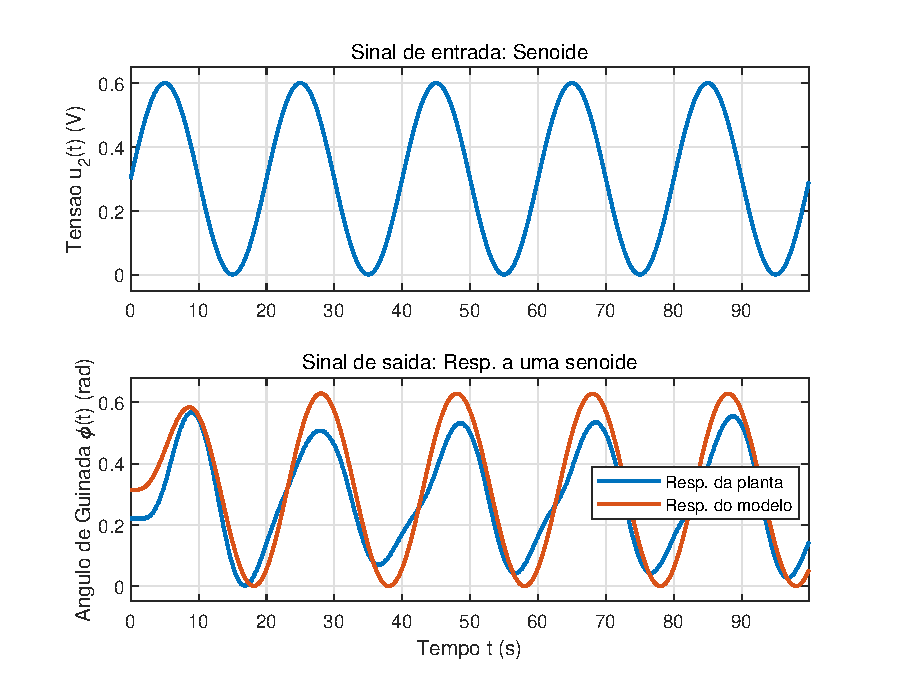
\includegraphics[width=0.48\textwidth]{figures/Validacao/ValidaYawSenoide.eps}
    \caption{\textit{Yaw}: Sinal de entrada senoidal e resposta da planta e do modelo a essa entrada.}
    \label{fig:ValidaYawSenoide}
\end{figure}

Observa-se que o modelo seguiu o comportamento original da planta, em termos de frequência de oscilação, destoando um pouco apenas na amplitude.

%%%%%%%%%%%%%%%%%%%%%%%%%%%%%%%%%%%%%%%%%%%%%%%%%%%%%%%%%%%%%%%%%%%
\subsection{\textbf{Validação do Modelo do \textit{cross-pitch}}}

A validação do modelo obtido para o \textit{cross-pitch} para sinais de entrada do tipo pulso e senoide, são apresentados nas Figuras \ref{fig:ValidaCrossPitchPulso} e \ref{fig:ValidaCrossPitchSenoide}.

Na Figura \ref{fig:ValidaCrossPitchPulso}, foi aplicado um pulso de amplitude $\pm \SI{0.5}{\volt}$, com frequência de $f = 1/\SI{50}{\s} = \SI{0.02}{\Hz}$.

\begin{figure}[H]
    \centering
    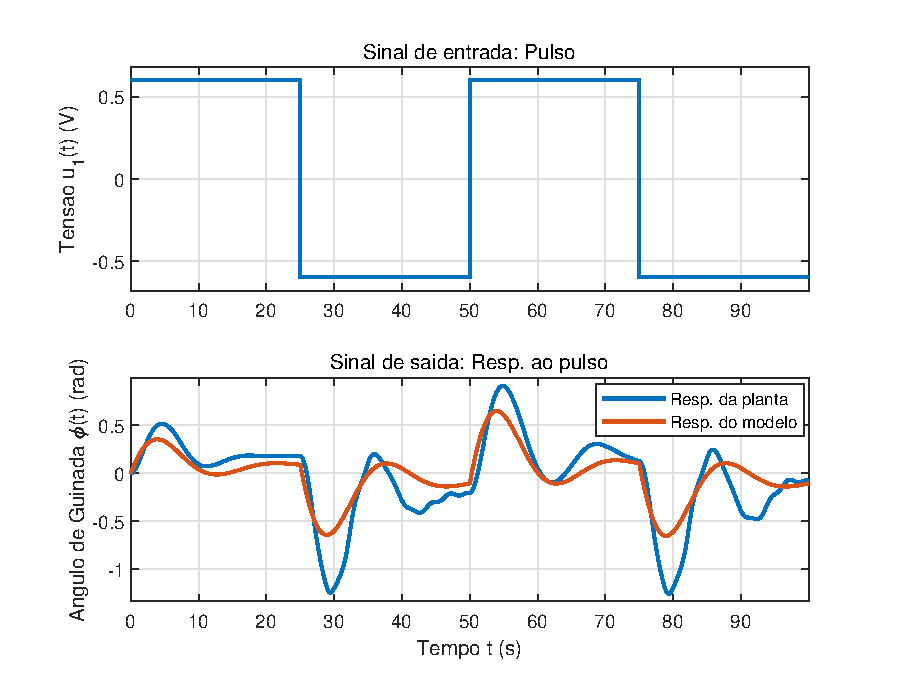
\includegraphics[width=0.48\textwidth]{figures/Validacao/ValidaCrossPitchPulso.eps}
    \caption{\textit{Cross-pitch}: Sinal de entrada em pulso e resposta da planta e do modelo a essa entrada.}
    \label{fig:ValidaCrossPitchPulso}
\end{figure}

Para amplitudes positivas, o modelo se aproximou melhor do comportamento real do sinal. 

Na Figura \ref{fig:ValidaCrossPitchSenoide}, foi aplicado um sinal senoidal de amplitude $\pm \SI{0.3}{\volt}$, com período de $T = \SI{50}{\s}$.

\begin{figure}[H]
    \centering
    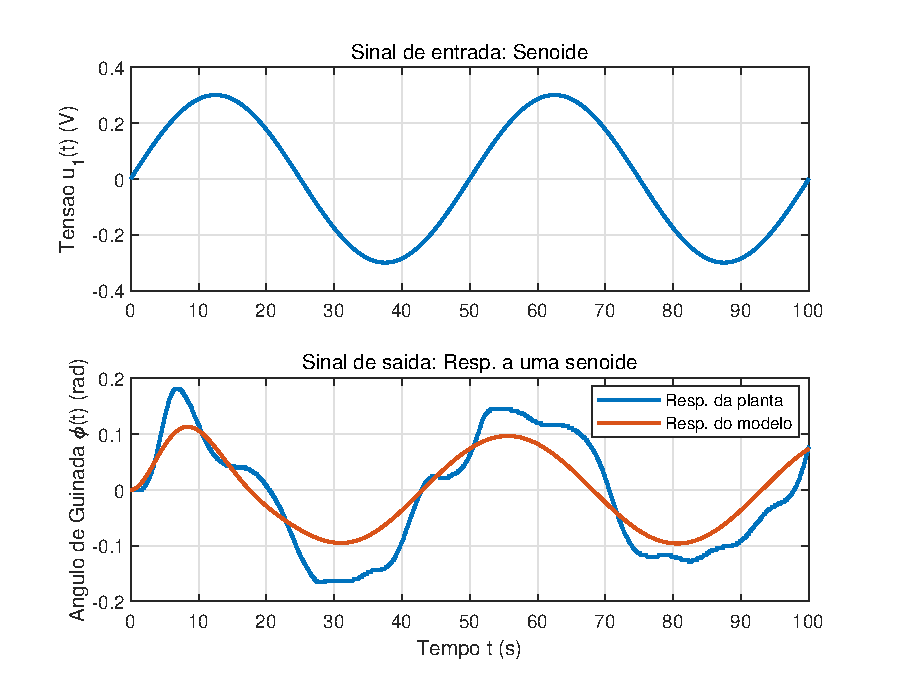
\includegraphics[width=0.48\textwidth]{figures/Validacao/ValidaCrossPitchSenoide.eps}
    \caption{\textit{Cross-pitch}: Sinal de entrada senoidal e resposta da planta e do modelo a essa entrada.}
    \label{fig:ValidaCrossPitchSenoide}
\end{figure}

Apesar das oscilações apresentadas pelo sinal original da planta, observa-se que o modelo foi capaz de seguir de forma razoável a trajetória correta.

%%%%%%%%%%%%%%%%%%%%%%%%%%%%%%%%%%%%%%%%%%%%%%%%%%%%%%%%%%%%%%%%%%%
\subsection{\textbf{Validação do Modelo do \textit{cross-yaw}}}

Na Figura \ref{fig:ValidaCrossYawPulso} é mostrada a resposta original da planta e a resposta do modelo para uma entrada em pulso com amplitude $\pm \SI{0.4}{\volt}$.

\begin{figure}[H]
    \centering
    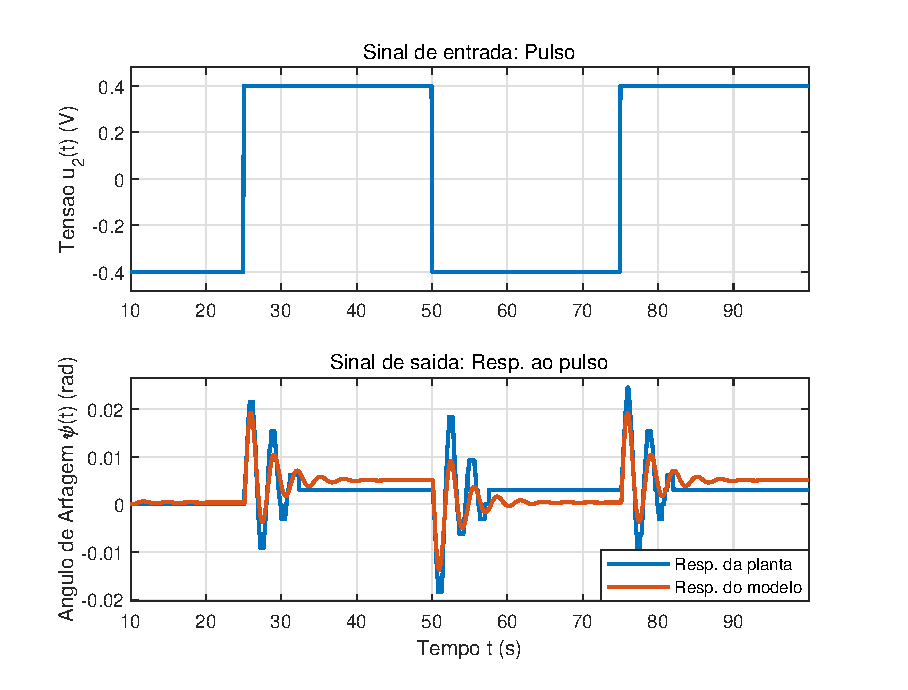
\includegraphics[width=0.48\textwidth]{figures/Validacao/ValidaCrossYawPulso.eps}
    \caption{\textit{Cross-yaw}: Sinal de entrada em pulso e resposta da planta e do modelo a essa entrada.}
    \label{fig:ValidaCrossYawPulso}
\end{figure}

Devido a baixa amplitude da resposta, da ordem de $\SI{e-3}{}$, e a impossibilidade de se aumentar a amplitude do sinal de entrada, devido a excursão limitada do giro do rotor, outros sinais de entrada não foram testados. Além disso, o período de amostragem, de $T_{s} = \SI{0.001}{\s}$, não pode ser reduzido ainda mais para se obter melhores resoluções, pois ao fazer isso, a quantidade de pontos de simulação era drasticamente reduzida.

\section{Desacoplamento}\label{Sec:Desacopla}
	
Para que seja possível controlar os dois rotores por meio de controladores PID ou por realimentação de estados, é necessário desacoplar os sistemas. Isso é obtido reduzindo-se a influência que as FTs do \textit{cross-pitch} e \textit{cross-yaw} desempenham sobre o comportamento resultante dos ângulos de arfagem e guinada. Assim, esta seção busca descrever o projeto de desacoplamento adotado, bem como sua validação, em malha aberta, por meio de simulação.

\subsection{\textbf{Projeto dos Desacopladores}}

De acordo com \cite{seborg2010process}, o desacoplamento dos sistemas pode ser realizado projetando-se FTs $T_{12}(s)$ e $T_{21}(s)$ de forma que, quando conectadas ao sistema, como mostrado na Figura \ref{fig:ProjetoDesacopla}, sejam cancelados ou atenuados os efeitos de $G_{cp}(s)$ e de $G_{cy}(s)$.

\begin{figure}[H]
    \centering
    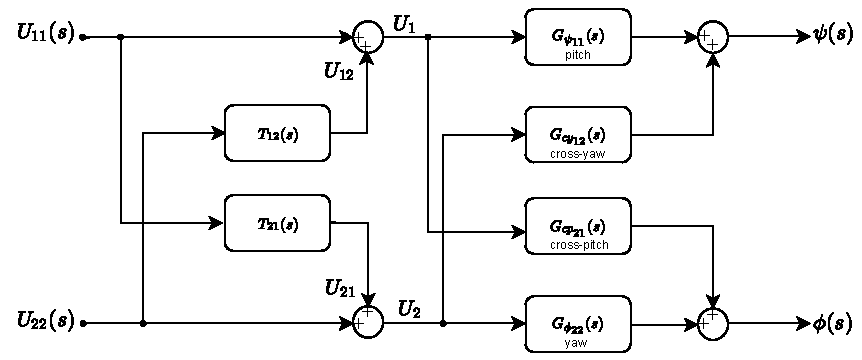
\includegraphics[width=0.48\textwidth]{figures/Desacoplamento/Desacoplamento.pdf}
    \caption{Diagrama de blocos do sistema MIMO com desacopladores.}
    \label{fig:ProjetoDesacopla}
\end{figure}

Assumindo-se inicialmente, que $U_{22} = 0$ e que $U_{11} \neq 0$, tem-se que
\begin{equation}\label{eq:T21}
    U_{21} = T_{21} U_{11}
\end{equation}
\noindent para desacoplar $G_{21}$, deve-se obter
\begin{equation}\label{eq:DesG21}
    U_{11} G_{21} + U_{21} G_{22} = 0
\end{equation}
\noindent substituindo \eqref{eq:T21} em \eqref{eq:DesG21} e isolando-se $T_{21}$:
\begin{equation}\label{eq:DesT21}
    T_{21} = - \frac{G_{21}}{G_{22}}
\end{equation}
Substituindo as FTs \eqref{eq:FTModeloIDCrossPitch} $G_{21}$ e \eqref{eq:FTModeloIDYaw} $G_{22}$ em \eqref{eq:DesT21FT}, obtém-se
\begin{equation}\label{eq:DesT21FT}
    T_{21} = - \frac{0.024987 (s+0.5231) (s^2 + 0.2437s + 4.123)}{s^2 + 0.6339s + 4.262}
\end{equation}
Aplicando-se o mesmo processo, agora para $U_{11} = 0$ e $U_{22} \neq 0$, é possível obter uma expressão para $T_{12}$ que desacopla $G_{12}$:
\begin{equation}\label{eq:T12}
    U_{12} = T_{12} U_{22}
\end{equation}
\begin{equation}\label{eq:DesG12}
    U_{22} G_{12} + U_{12} G_{11} = 0
\end{equation}
\noindent substituindo \eqref{eq:T12} em \eqref{eq:DesG12} e isolando-se $T_{12}$:
\begin{equation}\label{eq:DesT12}
    T_{12} = - \frac{G_{12}}{G_{11}}
\end{equation}
Substituindo as FTs \eqref{eq:FTModeloIDCrossYaw} $G_{12}$ e \eqref{eq:FTModeloIDPitch} $G_{11}$ em \eqref{eq:DesT12FT}, obtém-se
\begin{equation}\label{eq:DesT12FT}
    T_{12} = - \frac{0.8299 (s+0.06236) (s^2 + 0.3948s + 0.2209)}{s^2 + 0.2574s + 0.1437}
\end{equation}
Das equações \eqref{eq:DesT21FT} e \eqref{eq:DesT12FT} para $T_{12}$ e $T_{21}$, vê-se que foram obtidas equações não realizáveis na prática. Com base nisso, buscou-se aproximar essas equações desacoplamento apenas pelo seus ganhos estáticos. O que é equivalente a desacoplar os sistemas em regime permanente \cite{seborg2010process}.
\begin{equation}\label{eq:T21Gain}
    T_{{21}_{k}} = -0.024987
\end{equation}
\begin{equation}\label{eq:T12Gain}
    T_{{12}_{k}} = -0.829900
\end{equation}
Após ajustes desses ganhos com objetivo de melhorar o desacoplamento, obteve-se
\begin{equation}\label{eq:T21GainFinal}
    T_{{21}_{k}} = -0.05
\end{equation}
\begin{equation}\label{eq:T12GainFinal}
    T_{{12}_{k}} = -0.07
\end{equation}
Esses valores foram utilizados nas simulações de validação do desacoplamento, cujos resultados são mostrados na próxima seção.

\subsection{\textbf{Validação do Desacoplamento}}

A validação do desacoplamento projetado foi realizada por meio da aplicação de dois sinais de entrada: um do tipo pulso e uma senoide. Foram analisados os sinais do \textit{pitch} e \textit{yaw}, \textit{cross-pitch} e \textit{cross-yaw}, assim como da soma de \textit{cross-yaw} com \textit{pitch} e \textit{cross-pitch} com o \textit{yaw}. A ideia foi a de mostrar que a influência das FTs do \textit{cross-pitch} e \textit{cross-yaw} foram reduzidas após a inserção dos desacopladores, fazendo com que o sinal proveniente da soma e o sinal direto ficassem mais próximos.

%%%%%%%%%%%%%%%%%%%%%%%%%%%%%%%%%%%%%%%% PITCH

Na Figuras \ref{fig:PitchAcopladoPulso}, \ref{fig:PitchDesacopladoPulso}, \ref{fig:PitchAcopladoSenoide} e \ref{fig:PitchDesacopladoSenoide} são mostrados os resultados da aplicação dos sinais mencionados para o \textit{pitch}, mostrando o comportamento dos sinais antes (acoplados) e após (desacoplados).

\begin{figure}[H]
    \centering
    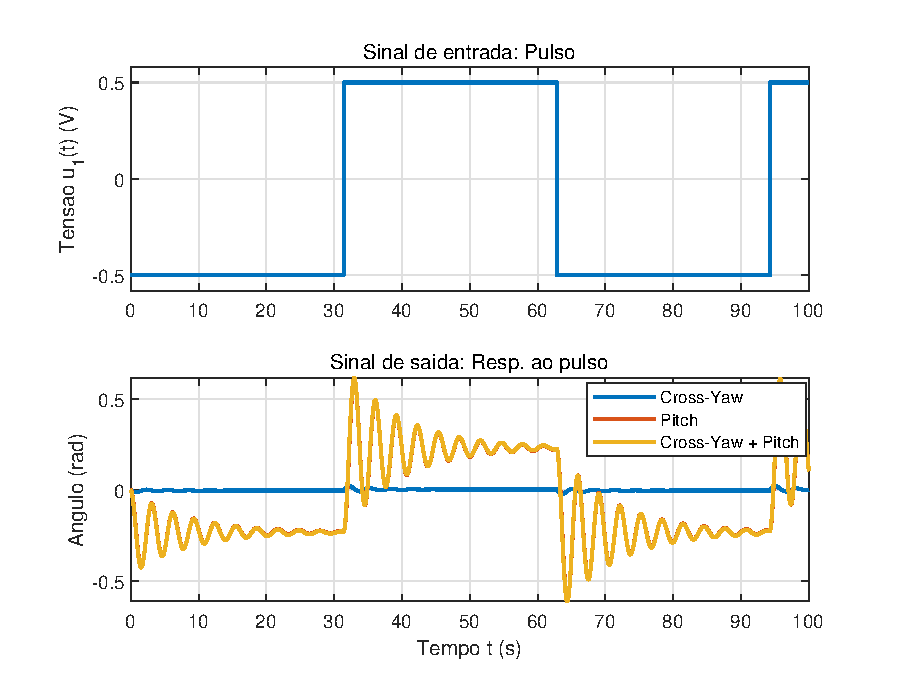
\includegraphics[width=0.48\textwidth]{figures/Desacoplamento/Pitch_Acoplado_Pulso.eps}
    \caption{Ângulo do \textit{pitch}: Acoplado.}
    \label{fig:PitchAcopladoPulso}
\end{figure}

\begin{figure}[H]
    \centering
    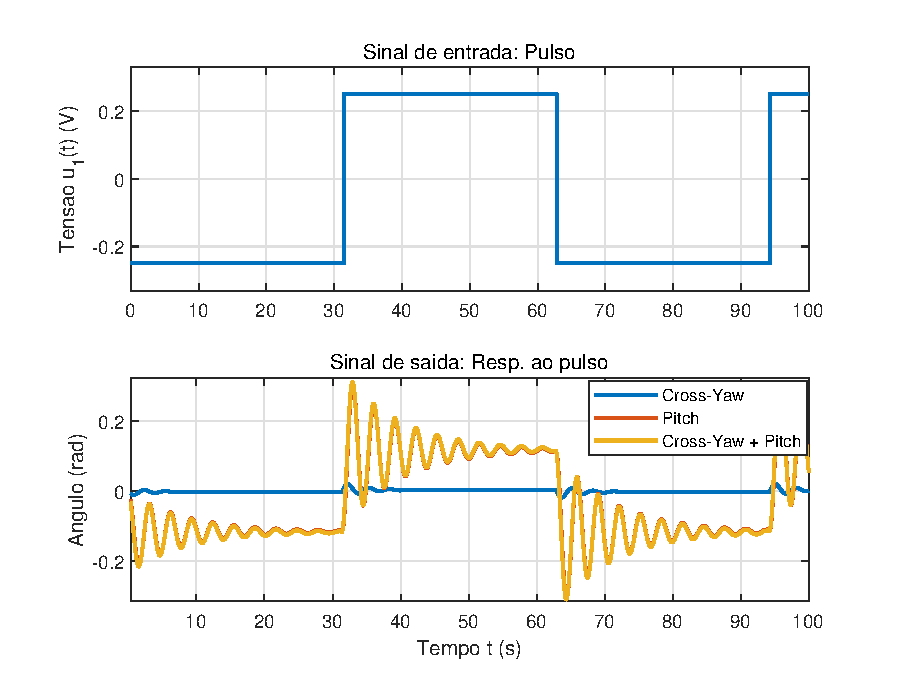
\includegraphics[width=0.48\textwidth]{figures/Desacoplamento/Pitch_Desacoplado_Pulso.eps}
    \caption{Ângulo do \textit{pitch}: Desacoplado.}
    \label{fig:PitchDesacopladoPulso}
\end{figure}

\begin{figure}[H]
    \centering
    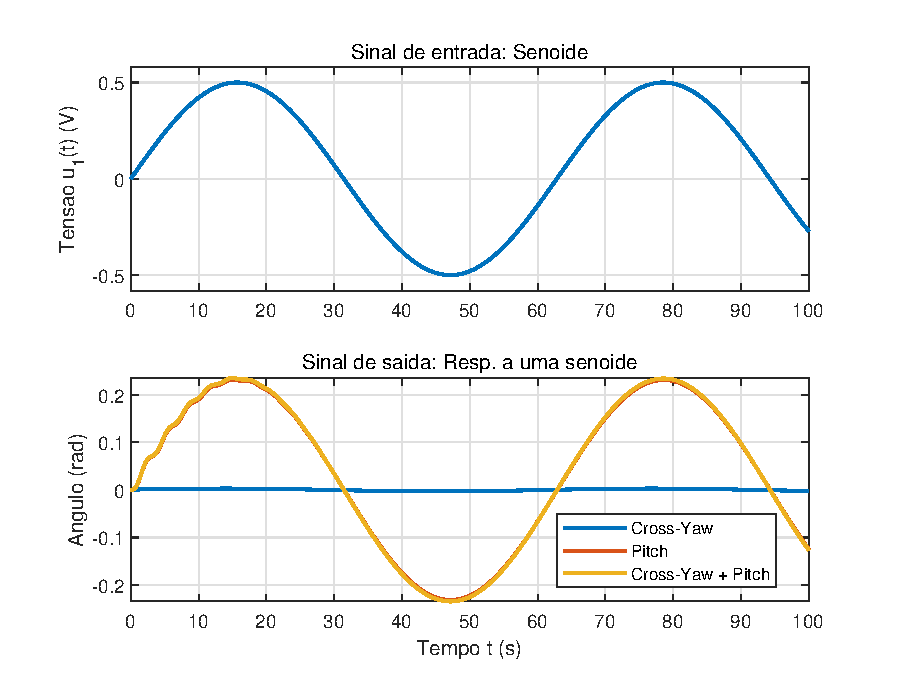
\includegraphics[width=0.48\textwidth]{figures/Desacoplamento/Pitch_Acoplado_Senoide.eps}
    \caption{Ângulo do \textit{pitch}: Acoplado.}
    \label{fig:PitchAcopladoSenoide}
\end{figure}

\begin{figure}[H]
    \centering
    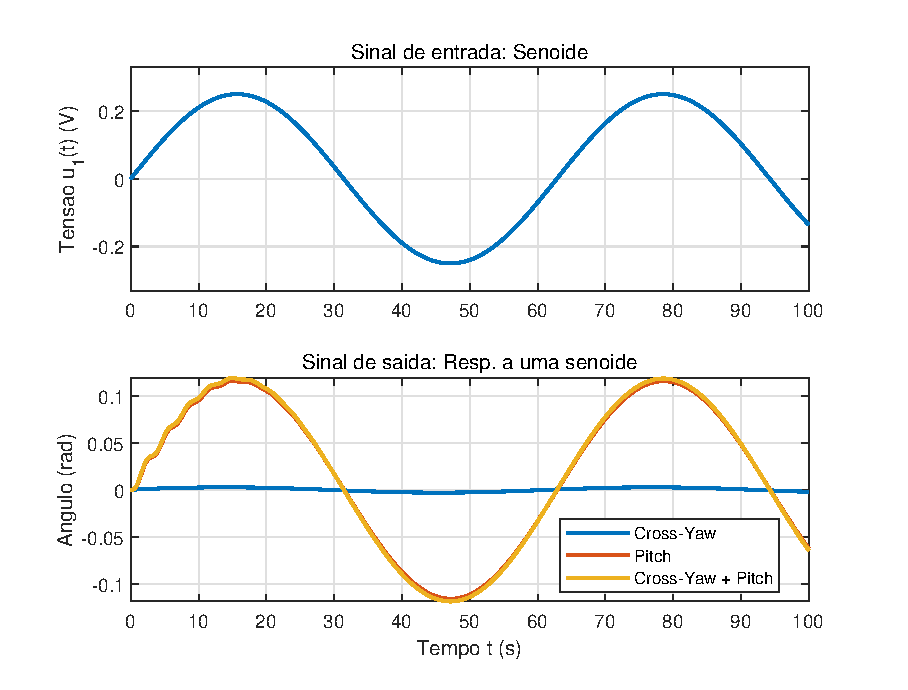
\includegraphics[width=0.48\textwidth]{figures/Desacoplamento/Pitch_Desacoplado_Senoide.eps}
    \caption{Ângulo do \textit{pitch}: Desacoplado.}
    \label{fig:PitchDesacopladoSenoide}
\end{figure}

Para os dois tipos de sinais aplicados, vê-se que o comportamento do ângulo do \textit{pitch} não melhorou de forma perceptiva. Isso se deve ao fato de que a influência da FT do \textit{cross-yaw} ser muito pequena, como pode ser observado nas Figuras \ref{fig:IdentificacaoCrossYawInicial} e \ref{fig:IdentificacaoCrossYawFinal}, obtidas no processo de identificação do modelo, nas quais o ganho da FT é da ordem de $\SI{1e-3}{}$.

%%%%%%%%%%%%%%%%%%%%%%%%%%%%%%%%%%%%%%%% YAW

Na Figuras \ref{fig:YawAcopladoPulso}, \ref{fig:YawDesacopladoPulso}, \ref{fig:YawAcopladoSenoide} e \ref{fig:YawDesacopladoSenoide} são mostrados os resultados obtidos antes e após o desacoplamento dos ângulos.

\begin{figure}[H]
    \centering
    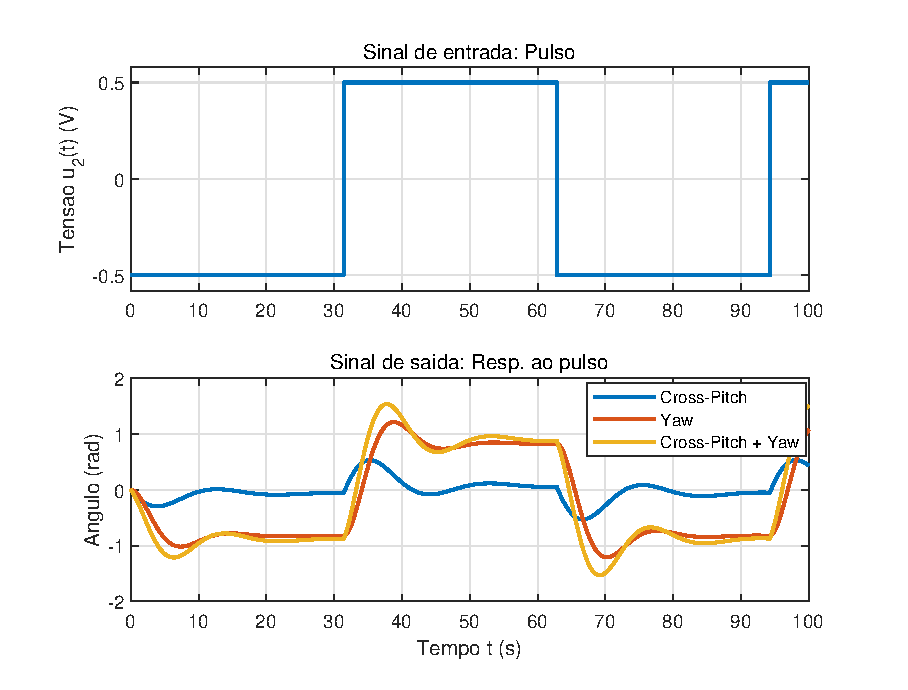
\includegraphics[width=0.48\textwidth]{figures/Desacoplamento/Yaw_Acoplado_Pulso.eps}
    \caption{Ângulo do \textit{yaw}: Acoplado.}
    \label{fig:YawAcopladoPulso}
\end{figure}

\begin{figure}[H]
    \centering
    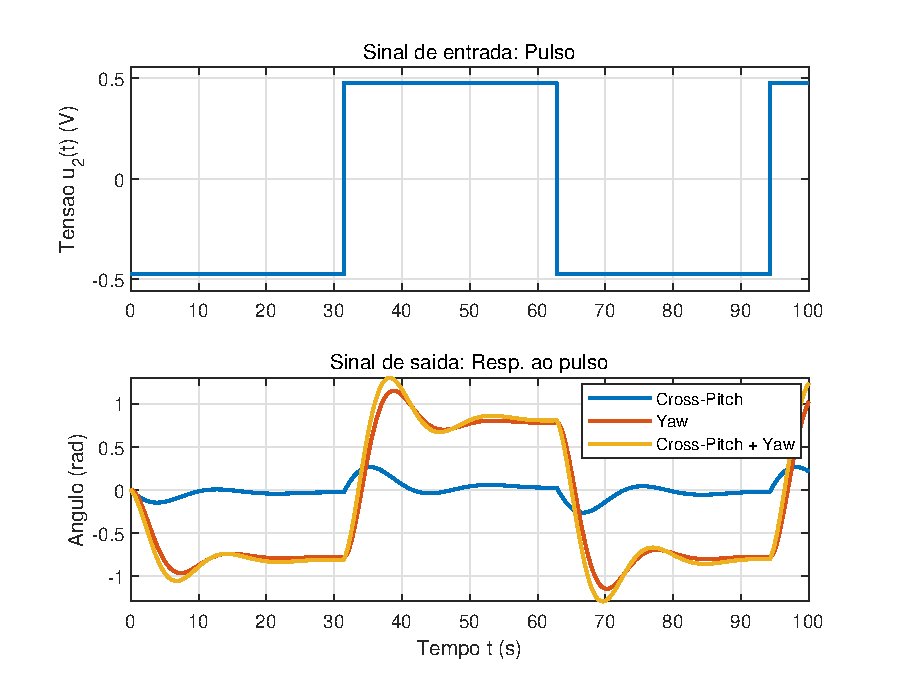
\includegraphics[width=0.48\textwidth]{figures/Desacoplamento/Yaw_Desacoplado_Pulso.eps}
    \caption{Ângulo do \textit{yaw}: Desacoplado.}
    \label{fig:YawDesacopladoPulso}
\end{figure}


\begin{figure}[H]
    \centering
    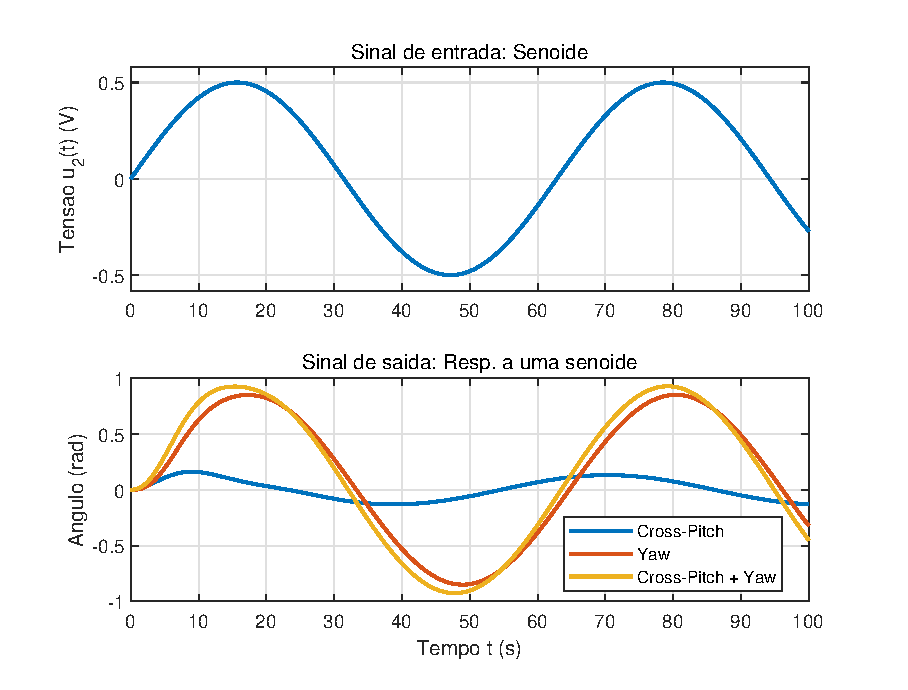
\includegraphics[width=0.48\textwidth]{figures/Desacoplamento/Yaw_Acoplado_Senoide.eps}
    \caption{Ângulo do \textit{yaw}: Acoplado.}
    \label{fig:YawAcopladoSenoide}
\end{figure}

\begin{figure}[H]
    \centering
    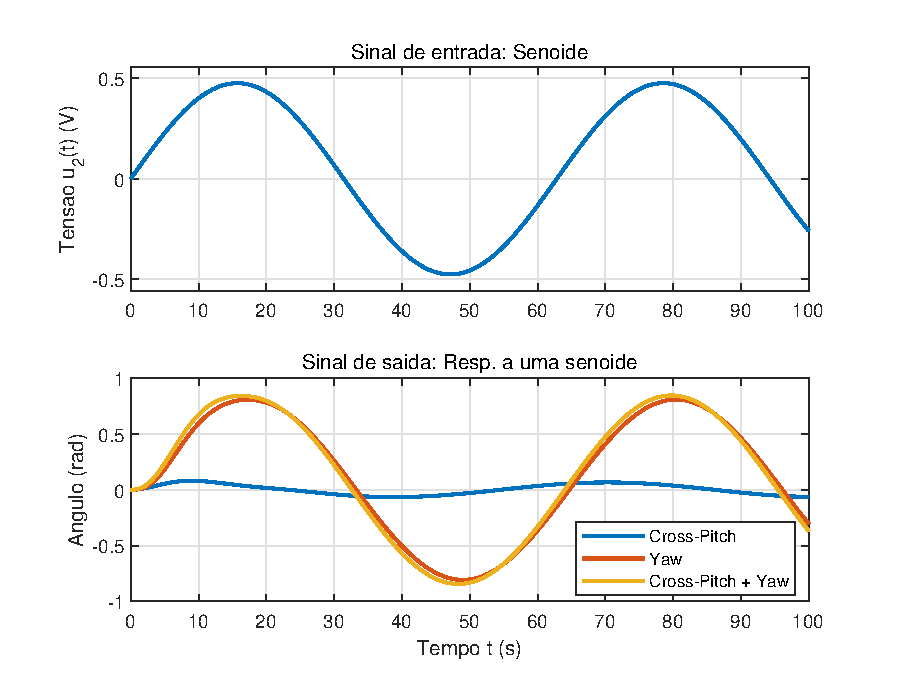
\includegraphics[width=0.48\textwidth]{figures/Desacoplamento/Yaw_Desacoplado_Senoide.eps}
    \caption{Ângulo do \textit{yaw}: Desacoplado.}
    \label{fig:YawDesacopladoSenoide}
\end{figure}

Ao contrário do observado para o \textit{pitch}, vê-se que o desacoplamento foi capaz de reduzir a influência do \textit{cross-pitch} à aproximadamente a metade, com seu valor máximo de pico reduzindo de $\approx 0.5$ para $\approx 0.25$ (Figuras \ref{fig:YawAcopladoPulso} e \ref{fig:YawDesacopladoPulso}). A redução do acoplamento é percebida também na aplicação do sinal senoidal.

\section{Controle por Realimentação de Estados}\label{Sec:ControleEE}
	
Nesta seção são descritas as etapas do projeto de um controlador por realimentação de estados para uma representação do sistema MIMO em espaço de estados. Inicialmente, é mostrada a conversão do sistema de FTs para espaço de estados, seguida da alteração das matrizes $C$ e $D$ para permitir a realimentação de todos os estados. Em seguida, são especificados os polos de malha fechada desejados e um controlador por realimentação de estados é obtido.

Inicialmente, obteve-se a matriz de FT do sistema MIMO, dada por:
$$ \begin{bmatrix}
        Y_{p}(s)\\
        Y_{Y}(s)\\
        \end{bmatrix} = \begin{bmatrix}
        G_{11} & G_{12}\\
        G_{12} & G_{22}\\
        \end{bmatrix}
        \begin{bmatrix}
        U_{1}(s)\\
        U_{2}(s)\\
        \end{bmatrix} $$

Em seguida, obteve-se sua representação em espaço de estados, obtendo-se
\begin{align*}
    \dot{x} &= A x + B u \\
    Y &= C x + D u
\end{align*}
\noindent onde
$$ A = \scalemath{0.92}{\begin{bmatrix}
        -0.2 & -2.1 & 0 & 0 & 0 & 0 & 0 & 0\\
        2 & 0 & 0 & 0 & 0 & 0 & 0 & 0 \\
        0 & 0 & -0.3 & -0.3 & 0 & 0 & 0 & 0 \\
        0 & 0 & 0.5 & 0 & 0 & 0 & 0 & 0 \\
        0 & 0 & 0 & 0 & -0.6 & -2.1 & 0 & 0 \\
        0 & 0 & 0 & 0 & 2 & 0 & 0 & 0 \\
        0 & 0 & 0 & 0 & 0 & 0 & -0.4 & -0.4 \\
        0 & 0 & 0 & 0 & 0 & 0 & 0.5 & 0 \\
        \end{bmatrix} }$$
        
$$ B = \begin{bmatrix}
        1 & 0 \\
        0 & 0 \\
        0.5 & 0 \\
        0 & 0 \\
        0 & 0.25 \\
        0 & 0 \\
        0 & 1 \\
        0 & 0 \\
        \end{bmatrix} $$

$$ C = \begin{bmatrix}
        0 & 0.95 & 0 & 0 & 0.19 & 0.05 & 0 & 0 \\
        0 & 0 & 0.6 & 0.07 & 0 & 0 & 0 & 0.7 \\
        \end{bmatrix} $$

$$ D = \begin{bmatrix}
        0 & 0 \\
        0 & 0 \\
        \end{bmatrix} $$

A resposta ao degrau do sistema em espaço de estados retornou o resultado mostrado na Figura \ref{fig:StepResponseEEModel}.

\begin{figure}[H]
    \centering
    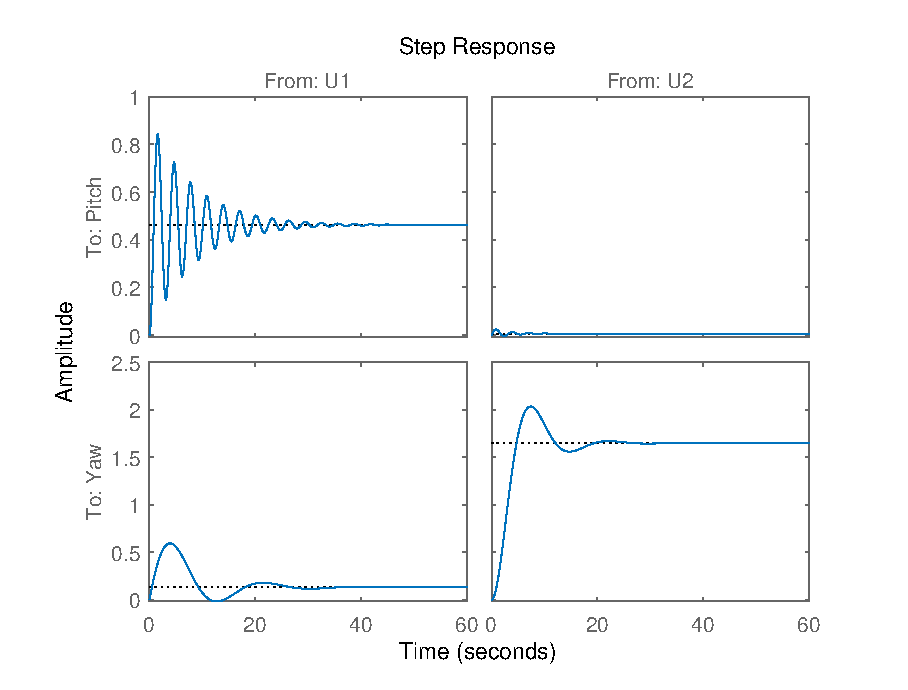
\includegraphics[width=0.48\textwidth]{figures/ControleEE/step_respons_ssmodel.eps}
    \caption{Resposta ao degrau do sistema MIMO em espaço de estados.}
    \label{fig:StepResponseEEModel}
\end{figure}

Um controlador por realimentação de estados requer que $u = - Kx$:
\begin{align*}
    \dot{x} &= A x - B k x \\
    \dot{x} &= (A - Bk) x
\end{align*}
\noindent onde $k$ representa uma matriz de ganhos da realimentação.

Para obtê-la, foram definidos os polos desejados de MF, segundo as especificações. Os quais foram obtidos pela ferramenta \textit{sisotool} do Matlab. A matriz de ganhos $k$ foi então obtida por meio do comando \textit{place()} do Matlab, passando-se as matrizes $A$ e $B$ e a matriz de polos desejados, obtendo-se

$$ k = \begin{bmatrix}
        3.12 & -0.15 & 0.01 & 0 & 0 & 0 & -0.06 & -0.18 \\
    0.15 & -0.03 & -0.2 & -0.04 & 0 & 0 & 2.9 & 6.8 \\
        \end{bmatrix} $$

Na Figura \ref{fig:StepResponseEEMAMF} é mostrada uma comparação entre a resposta do sistema MIMO a um degrau unitário em malha aberta e a resposta em malha fechada, a partir da realimentação de todos os estados com a matriz de ganho obtida.

\begin{figure}[h]
    \centering
    \includegraphics[width=0.48\textwidth]{figures/ControleEE/step_respons_allstates_MF_MA.eps}
    \caption{Resposta do sistema MIMO em MA e MF, considerando todos os estados da representação.}
    \label{fig:StepResponseEEMAMF}
\end{figure}

Para mapear de volta para as saídas desejadas, que relacionam o \textit{pitch} e o \textit{yaw} com as entradas $u_{1}$ e $u_{2}$, basta utilizar os ganhos presentes na matriz $B$.


\section{Controle PID}\label{Sec:ControlePID}
	Considerando a influência do cross-pitch e cross-yaw, e implementando o desacoplamento, obtemos um diagrama de controle correspondente a figura \ref{fig:ControleMIMOPID}. Para um sistema já desacoplado, resta realizar o controle isolado de cada grandeza a ser controlada da planta.

\begin{figure}[H]
    \centering
    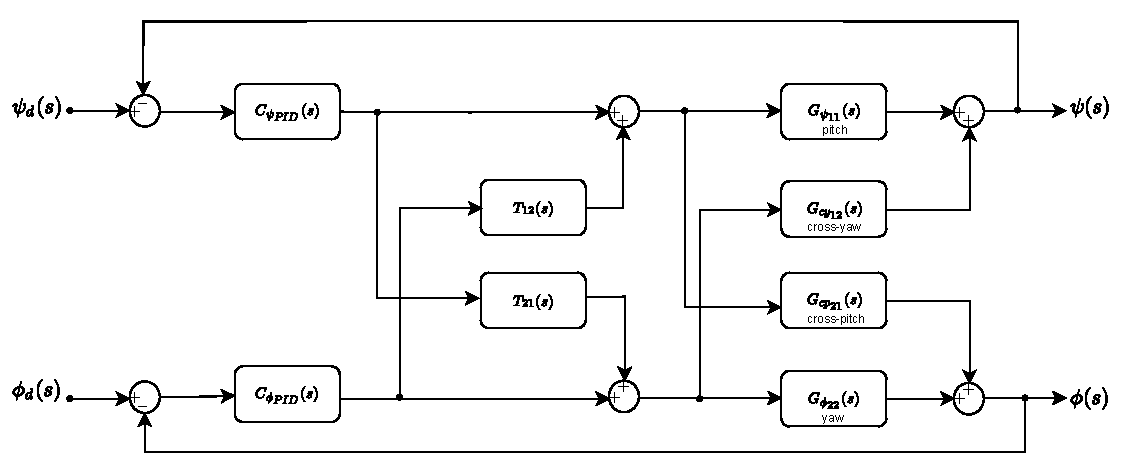
\includegraphics[width=0.48\textwidth]{figures/Controle/Controle_PID_Desacoplado.pdf}
    \caption{Diagrama de blocos do sistema MIMO com desacopladores e controladores PID para o \textit{yaw} e o \textit{pitch}.}
    \label{fig:ControleMIMOPID}
\end{figure}


Para realizar o controle de arfagem e guinada, projetou-se, por meio dos método do lugar das raízes, um controlador, seguindo os requisitos de desempenho apresentados na seção 2. O ganho foi ajustado iterativamente de forma a reduzir a ação de controle, via simulações, para que esta não atinja a saturação de 2.5V.
As figuras \ref{fig:rLocusPitch} e  \ref{fig:rLocusYaw} apresentam o lugar das raízes do PID para o controle de pitch e de yaw.

\begin{figure}[H]
    \centering
    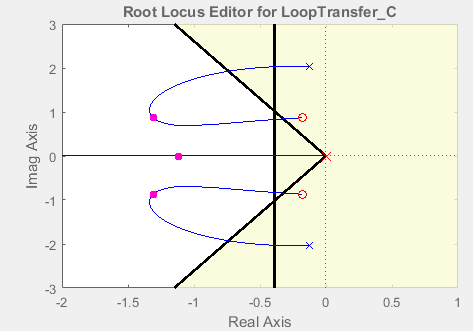
\includegraphics[width=0.48\textwidth]{figures/rlocus_MF.PNG}
    \caption{Lugar das raízes de um controlador PID para o controle do  \textit{pitch}.}
    \label{fig:rLocusPitch}
\end{figure}

\begin{figure}[H]
    \centering
    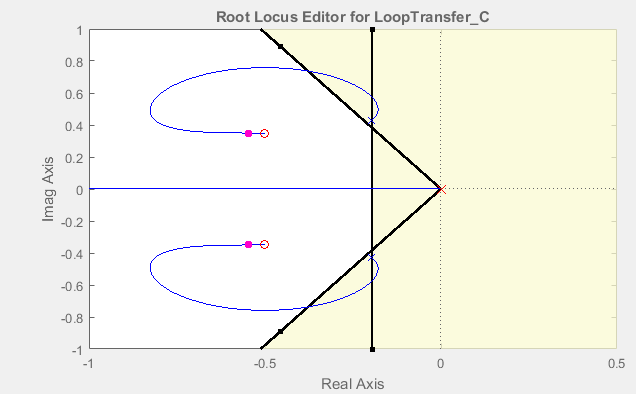
\includegraphics[width=0.48\textwidth]{figures/controlador_yaw_root_locus.PNG}
    \caption{Lugar das raízes de um controlador PID para o controle do  \textit{pitch}.}
    \label{fig:rLocusYaw}
\end{figure}


O controlador PID obtido para o pitch é dado pela equação \eqref{eq:PIDpitch}
\begin{equation}\label{eq:PIDpitch}
    C(s) = \frac{1.8 s^2 + 0.648 s + 0.789}{s}
\end{equation}


O controlador PID obtido para o yaw é dado pela equação \eqref{eq:PIDyaw}
\begin{equation}\label{eq:PIDyaw}
    C(s) = \frac{6.13 s^2 + 6.13 s + 3}{s}
\end{equation}

\section{Resultados Experimentais em MF}\label{Sec:ResultadosMF}
	
\subsection{\textbf{Teste do Controlador na Planta}}

Simulamos os controladores, até que estivessem com um desempenho satisfatório. Então foram realizados ensaios com uma entrada variável, para realizar a observação de desempenho dos controles com desacoplamento, correspondentes às figuras \ref{fig:ResultadosYaw}, \ref{fig:ResultadosPitch}.
É possível observar que o desempenho foi satisfatório e condizente com os requisitos.

\begin{figure}[H]
    \centering
    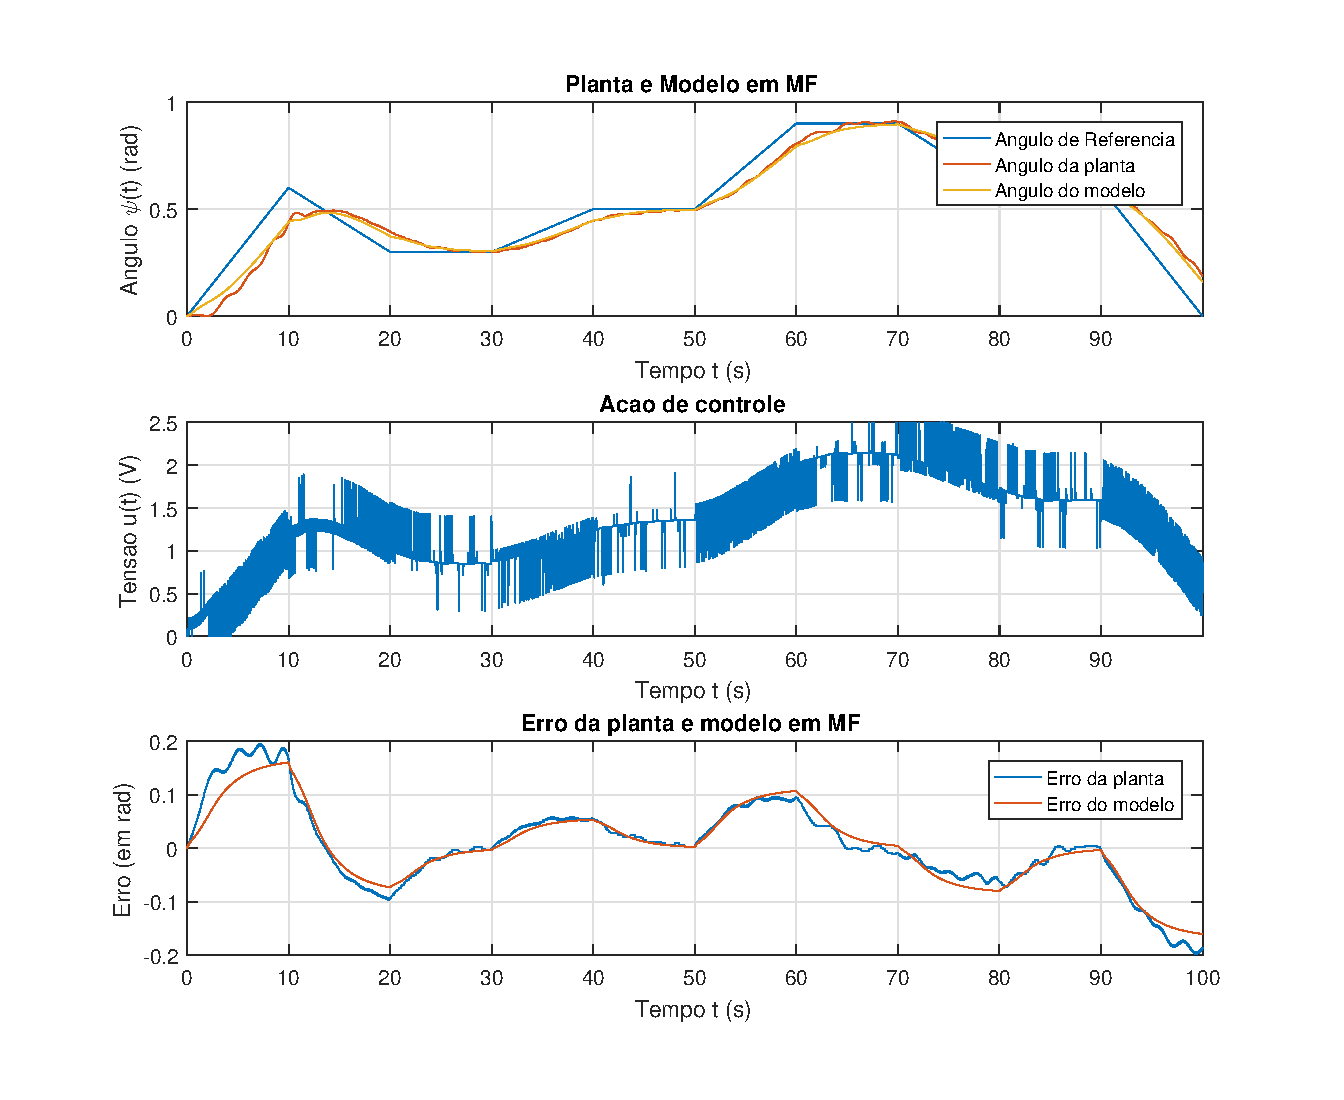
\includegraphics[width=0.5\textwidth]{figures/resultados/valida_pitch.eps}
    \caption{Validação de controle desacoplado de  \textit{pitch}.}
    \label{fig:ResultadosPitch}
\end{figure}

\begin{figure}[H]
    \centering
    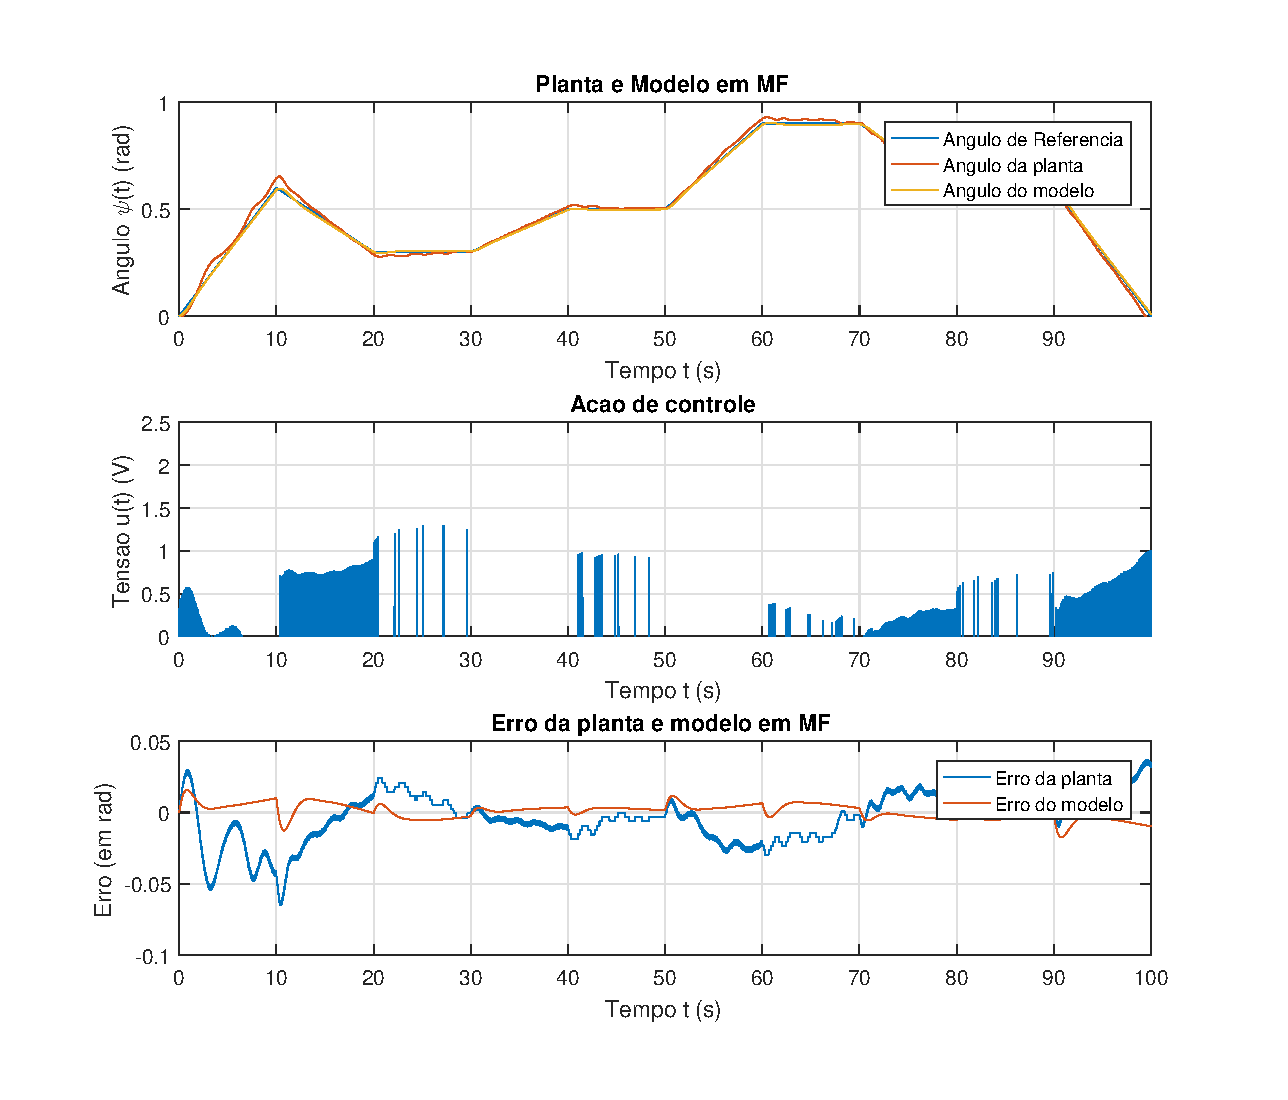
\includegraphics[width=0.5\textwidth]{figures/resultados/valida_yaw.eps}
    \caption{Validação de controle desacoplado de  \textit{yaw}.}
    \label{fig:ResultadosYaw}
\end{figure}


\subsection{\textbf{Análise de Desempenho}}

Para a avaliação de desempenho do sistema em malha fechada para a entrada variável mostrada na Figura \ref{fig:ValidaControladorEntradaVariavel}, foi realizada utilizando-se dois índices de desempenho, a Integral do Erro Quadrático (\textit{ISE - Integral Squared Error}) e a Integral do Erro Absoluto (\textit{IAE - Integral Absolute Error}). Os quais foram calculados por meio das equações \eqref{eq:ISE} e \eqref{eq:IEA}
 \begin{equation}\label{eq:ISE}
     ISE = \int_{0}^{T} e^{2}(t) dt
 \end{equation}
 \begin{equation}\label{eq:IEA}
     IEA = \int_{0}^{T} |e(t)| dt
 \end{equation}

\noindent onde $e$ é o erro, dado pela diferença entre o \textit{set-point} e o ângulo medido e $T$ representa a janela de tempo considerada.
 
Para o \textit{yaw}, obtivemos os seguintes índices:
$$ISE = 2.8430 $$
$$IAE = \SI{450.3624}{} $$
E para o \textit{pitch}, obtivemos:
$$ISE = 507.7020 $$
$$IAE = \SI{5.5331e+03}{} $$


	
\section{Conclusões}\label{Sec:ConsiderFinais}
	Por meio dessa prática, foi possível controlar, com desempenho satisfatório, uma planta do tipo MIMO, utilizando a técnica de desacoplamento, dessa forma possibilitando o controle para yaw e pitch independentemente. 

\bibliography{reference}
\bibliographystyle{apalike}

\end{document}
